% This must be in the first 5 lines to tell arXiv to use pdfLaTeX, which is strongly recommended.
\pdfoutput=1
% In particular, the hyperref package requires pdfLaTeX in order to break URLs across lines.

\documentclass[11pt]{article}

% Remove the "review" option to generate the final version.
\usepackage{acl}

% Standard package includes
\usepackage{times}
\usepackage{latexsym}

% For proper rendering and hyphenation of words containing Latin characters (including in bib files)
\usepackage[T1]{fontenc}
% For Vietnamese characters
% \usepackage[T5]{fontenc}
% See https://www.latex-project.org/help/documentation/encguide.pdf for other character sets

% This assumes your files are encoded as UTF8
\usepackage[utf8]{inputenc}

% This is not strictly necessary, and may be commented out,
% but it will improve the layout of the manuscript,
% and will typically save some space.
\usepackage{microtype}

% If the title and author information does not fit in the area allocated, uncomment the following
%
%\setlength\titlebox{<dim>}
%
% and set <dim> to something 5cm or larger.

\usepackage{tcolorbox}
\usepackage{arydshln}
\usepackage{algorithm}
\usepackage{algpseudocode}
\usepackage{ulem}
\usepackage{soul}
\usepackage{xcolor}
\usepackage{todonotes}
\definecolor{mybluei}{RGB}{0,173,239}

\renewcommand{\algorithmicensure}{\textbf{Output:~}}

\usepackage{xspace}
\newcommand{\method}{\mbox{\textsc{TRACER}}\xspace}

\algnewcommand{\LeftComment}[1]{\Statex \(\triangleright\) #1}

\makeatletter
\def\els@aparagraph[#1]#2{\elsparagraph[#1]{#2}}
\def\els@bparagraph#1{\elsparagraph*{#1}}
\makeatother

\title{Wizard of Shopping: Target-Oriented E-commerce Dialogue Generation with Decision Tree Branching}

% Author information can be set in various styles:
% For several authors from the same institution:
% \author{Author 1 \and ... \and Author n \\
%         Address line \\ ... \\ Address line}
% if the names do not fit well on one line use
%         Author 1 \\ {\bf Author 2} \\ ... \\ {\bf Author n} \\
% For authors from different institutions:
% \author{Author 1 \\ Address line \\  ... \\ Address line
%         \And  ... \And
%         Author n \\ Address line \\ ... \\ Address line}
% To start a seperate ``row'' of authors use \AND, as in
% \author{Author 1 \\ Address line \\  ... \\ Address line
%         \AND
%         Author 2 \\ Address line \\ ... \\ Address line \And
%         Author 3 \\ Address line \\ ... \\ Address line}

% \author{First Author \\
%   Affiliation / Address line 1 \\
%   Affiliation / Address line 2 \\
%   Affiliation / Address line 3 \\
%   \texttt{email@domain} \\\And
%   Second Author \\
%   Affiliation / Address line 1 \\
%   Affiliation / Address line 2 \\
%   Affiliation / Address line 3 \\
%   \texttt{email@domain} \\}

\author{Xiangci Li\textsuperscript{\rm 1}$^*$ ~~ Zhiyu Chen\textsuperscript{\rm 2} ~~ Jason Ingyu Choi\textsuperscript{\rm 2}
\AND Nikhita Vedula\textsuperscript{\rm 2} ~~ Besnik Fetahu\textsuperscript{\rm 2} ~~ Oleg Rokhlenko\textsuperscript{\rm 2} ~~ Shervin Malmasi\textsuperscript{\rm 2} \\
  \textsuperscript{\rm 1} AWS AI Labs 
  \textsuperscript{\rm 2} Amazon.com, Inc. \\
  \tt lixiangci8@gmail.com \\ \tt \{zhiyuche, chojson, veduln, besnikf, olegro, malmasi\}@amazon.com \\
}

\begin{document}
\maketitle

\def\thefootnote{*}\footnotetext{~Work performed by the author as a PhD candidate at The University of Texas at Dallas before joining AWS AI Labs.}
\def\thefootnote{\arabic{footnote}}

\begin{abstract}
The goal of conversational product search (CPS) is to develop an intelligent, chat-based shopping assistant that can directly interact with customers to understand shopping intents, ask clarification questions, and find relevant products. However, training such assistants is hindered mainly due to the lack of reliable and large-scale datasets. %Prior studies of CPS are often limited to a very restricted domain (e.g., movie recommendation), or rely on synthetic templates. One alternative is to crowd source high-quality conversations, but this is a nontrivial task given the data noise and steep costs involved.
% interact with a chat-based shopping agent to obtain product recommendations by narrowing down product requirements through dialogue based search. %Prior work on CPS has significant shortcomings. 
%Despite great potential, the development of CPS agents has been challenging. 
Prior human-annotated CPS datasets are extremely small in size and lack integration with real-world product search systems. %Prior studies on CPS focused on representation learning, where the conversations are primarily template-based, lack a natural flow, and are often restricted to fixed domains. %It is also unclear how to extend existing data generation models to a new product domain since these models are usually trained with a fixed dataset. 
We propose a novel approach, \method, which leverages large language models (LLMs) to generate realistic and natural conversations for different shopping domains. \method's novelty lies in grounding the generation to dialogue plans, which are product search trajectories predicted from a decision tree model, that guarantees relevant product discovery in the shortest number of search conditions. 
% collect the first ever large-scale, human-like, target-oriented CPS dataset, called \textit{Wizard-of-Shopping (WoS)}.
% There are three major challenges involved: (1) %Since LLMs are not directly trained with a product catalog, they do not have direct access to product metadata. 
% (1) LLMs are not directly trained with product catalogs and product metadata;
% (2) %LLMs struggle with how and when to ask effective clarification questions to assist customers in quickly discovering their desired products.
% LLMs do not understand when and how to ask clarification questions during search; and (3) %it is unclear how to model customer preferences without real-world shopping data. 
% LLMs can't personalize product searches based on different real-world user preferences. 
% To tackle these, we create dialogue plans that ground LLMs to generate product search conversations, by leveraging decision tree models to select product attributes that uncover the target products.
%we propose a novel \textbf{T}arget-oriented e-comme\textbf{R}ce di\textbf{A}logue generation approach with de\textbf{C}ision tr\textbf{E}e b\textbf{R}anching (\method). 
%It first samples product features to construct a user profile, by capturing elements that customers may or may not desire. Then, a conversation plan is created by selecting product attributes via interpretable decision tree models that are relevant to the target products. These plans are finally used to ground LLMs to generate product search conversations. %prompting techniques, we leverage the chosen attributes to ground LLM-generated conversations to the product catalog. This ensures the successful discovery of target products by the end of the conversations between users and LLMs. 
%We claim that our approach is domain-agnostic, and h
%Our main contributions are: (1) proposing a CPS approach, \method, that can generalize across different shopping domains; (2) 
We also release the first target-oriented CPS dataset \textit{Wizard of Shopping (WoS)}, containing highly natural and coherent conversations (3.6k) from three shopping domains. Finally, we demonstrate the quality and effectiveness of \textit{WoS} via human evaluations and downstream tasks.

% Human evaluations demonstrate that our generated conversations are highly natural and coherent. We further demonstrate the usefulness of our dataset by using it to train downstream conversational query generators and conversational product ranker models, that significantly outperform baselines.
\end{abstract}

\section{Introduction}
\label{sec:intro}
% Image editing methods in diffusion models depend on user-defined control directions - users can unlock their creativity using these methods by specifying the desired manipulation through prompts~\cite{gandikota2023concept}, reference images~\cite{ruiz2022dreambooth, kumari2022customdiffusion, gal2022image, chen2024trainingfreeregionalpromptingdiffusion}, or attribute vectors~\cite{parmar2023zero,hertz2022prompt}. In this work, we ask a fundamentally different question: \emph{Can we automatically discover the underlying visual structure of a concept within diffusion model's knowledge?} %Rather than requiring user-specified controls, we aim to decompose the model's internal knowledge into meaningful directions.

% This question touches on a fundamental limitation in how we interact with diffusion models. Current control methods ~\cite{zhang2023addingconditionalcontroltexttoimage, gandikota2023concept, ye2023ipadaptertextcompatibleimage,ye2023ipadaptertextcompatibleimage, hertz2024stylealignedimagegeneration, li2023photomaker, shi2024instantbooth, chen2024trainingfreeregionalpromptingdiffusion} require users to specify their desired manipulations in advance, limiting interactive creativity. This contrasts with natural human artistic workflows, where creators dynamically explore creative ideas while jointly refining them toward meaningful artistic outcomes~\cite{hoffmann2016modeling}. This synergy between specification and exploration is not new to generative models. Early GAN architectures naturally developed disentangled latent spaces that enabled continuous\cite{harkonen2020ganspace,radford2015unsupervised, wu2021stylespace, shen2020interfacegan}, compositional control over generated images. Users could explore these spaces to discover interesting variations that would be difficult to describe in words~\cite{wu2021stylespace}, then combine them to achieve their creative goals~\cite{grabe2022towards}. 


% While diffusion models have largely superseded GANs in conditional image synthesis~\cite{dhariwal2021diffusion},  their underlying structure remains less understood. Diffusion models achieve remarkable diversity through high-dimensional latents, unlike GANs' compact latent spaces.  With a single prompt, diffusion models can generate radically different variations through different random initializations of input noise. We ask - Is it possible to discover interpretable structure within this vast space of variations?

Text-to-image diffusion models are capable of generating remarkable visual variations from a single prompt through different random initializations. However, this vast creative potential remains largely opaque to users---while we can generate diverse images, we lack understanding of the underlying structure of these variations. This presents a fundamental challenge: how can we discover and expose the latent visual capabilities encoded within these models?

\let\thefootnote\relax \footnote{$^{*}$Correspondence to \texttt{gandikota.ro@northeastern.edu}}

The challenge touches on a key limitation in how we interact with diffusion models today. Current control methods require users to explicitly specify their desired edits in advance through prompts~\cite{gandikota2023concept}, reference images~\cite{zhang2023addingconditionalcontroltexttoimage, chen2024trainingfreeregionalpromptingdiffusion, ruiz2022dreambooth,kumari2022customdiffusion, Ryu_lora, hu2021lora}, or attribute vectors~\cite{ye2023ipadaptertextcompatibleimage, hertz2024stylealignedimagegeneration, li2023photomaker, shi2024instantbooth,parmar2023zero,hertz2022prompt}. That contrasts sharply with natural human creative workflows, where artists dynamically explore creative ideas and jointly refine them toward meaningful artistic outcomes~\cite{hoffmann2016modeling}. The need for pre-specified controls creates a barrier between users and the full creative potential of these models.

Interestingly, earlier generative models like GANs~\cite{gans,karras2019style,brock2018large} naturally developed more interpretable internal structures. Their compact latent spaces often exhibited emergent disentanglement~\cite{harkonen2020ganspace,radford2015unsupervised, wu2021stylespace, shen2020interfacegan}, enabling continuous and compositional control over generated images. Users could explore these spaces to discover interesting variations that would be difficult to describe in words~\cite{wu2021stylespace}, then combine them to achieve their creative goals~\cite{grabe2022towards}.

Diffusion models have largely superseded GANs in conditional image synthesis~\cite{dhariwal2021diffusion}, achieving greater diversity through much higher-dimensional latents. And yet an understanding of the underlying structure of these larger latent spaces has remained elusive. In this work, we ask a fundamental question: \emph{Can we automatically discover the visual structure within a diffusion model's knowledge of a concept?} Rather than requiring user-specified controls, we aim to decompose the model's internal representations into expressive directions that users can explore and combine.

To address these needs, we present \textbf{SliderSpace}, a framework that brings systematic explorability to diffusion models. Given just a text prompt, SliderSpace discovers a canonical set of meaningful, diverse, and controllable directions within the model's knowledge of that concept. Each direction is implemented as a low-rank adapter~\cite{hu2021lora} that can be scaled and composed with others, allowing users to explore and smoothly combine different aspects of variation, as shown in Figure~\ref{fig:intro}.

We ground SliderSpace discovery in three key requirements for meaningful decomposition of a diffusion model's visual manifold: 
\begin{enumerate}
    \item \textbf{Unsupervised Discovery:} The decomposition process should emerge from the intrinsic structure of the model's learned representation, rather than being guided by predefined attributes. This ensures we capture the true topology of the model's knowledge space rather than projecting our assumptions onto it.
    
    \item \textbf{Semantic Orthogonality:} Each discovered control must represent a distinct semantic direction. This is enforced in a semantic feature space, like CLIP, where every slider has an orthogonal effect in embeddings. This prevents discovering multiple controls that create similar semantic effects, making the system more efficient and easier.
    
    \item \textbf{Distribution Consistency:} Directions must induce consistent transformations across both random seeds and prompt variations. 
\end{enumerate}

These requirements naturally lead to our proposed framework, which we formalize in Section~\ref{sec:method}. As we show in our experiments, SliderSpace is architecture-agnostic, working with both conventional U-Net based models like Stable Diffusion~\cite{rombach2022high, rombach2022sd20, podell2023sdxl, turbo, dmd} and recent transformer-based architectures like Flux~\cite{flux}.

We demonstrate the expressiveness of SliderSpace through three applications: First, we show how SliderSpace can decompose high-level concepts into diverse and expressive components, revealing the natural axes of variation in the model's understanding. Second, we explore artistic style variation, where SliderSpace discovers directions that match or exceed the diversity of manually curated artist lists while being judged more useful by human evaluators. Finally, we show how SliderSpace can help reverse the mode collapse commonly observed in distilled diffusion models, restoring diversity while maintaining generation speed.

Beyond providing practical creative control, SliderSpace opens new avenues for understanding and utilizing the latent capabilities of diffusion models. By mapping these models' visual potential into intuitive, composable directions, we take a step toward making their creative possibilities more accessible and interpretable to users.

% Image editing methods in diffusion models unlock the creativity of users. In this work we ask an alternate question: \emph{Can we organize and expose what of the diffusion model is already capable of?}.
% Existing methods for controlling image generation typically require users to manually specify edit directions for desired changes. This process is time-consuming, requires technical expertise, and limits the spontaneity of the creative process. For instance, if a user wants to adjust the smile of a generated person, they must explicitly request this edit, often through imprecise prompt engineering or model fine-tuning. This approach of predefined controls or manual specifications restricts users from fully exploring the latent capabilities of the model. There may be interesting stylistic variations or attributes that the model can generate, but users have no easy way to discover or utilize these.

% Natural visual disentanglement was an emergent property in the latent space of Generative Adversarial Models (GANs) \cite{harkonen2020ganspace,radford2015unsupervised, wu2021stylespace, shen2020interfacegan}. In particular, it has been observed that StyleGAN~\cite{karras2019style} stylespace neurons offer detailed control over many meaningful aspects of images that would be difficult to describe in words~\cite{wu2021stylespace}. However, diffusion models do not share such a compact latent space~\cite{park2023unsupervised}; and efforts to uncover such a space in the semantic embeddings of the text conditioning have met with limited success \nik{Nick - is there a specific citation you were thinking about?}.

% In this work we introduce \textbf{SliderSpace}, which takes a step towards uncovering an analogous low dimensional representation of diffusion models' visual breadth; in essence treating the diffusion model as many generators sharing parameters, where a particular generator is defined by a specific prompt. For a given prompt we sample many random seeds (and optionally prompt expansions using an LLM), generate the corresponding images, and apply an off the shelf feature extractor (in this work CLIP, but our method can be applied to any differentiable feature extractor). We use PCA to analyze these features, and for each of the leading $k$ principal components we train a LoRA \cite{} which causes the diffusion model to produces images which increase the feature magnitude along that component when passed back through the same feature extractor. This leads to a 'Slider' for each principal component, because each LoRA can be scaled and applied to the original diffusion model, continuously varying those visual features in the generated results (as measured, in our case, by CLIP).

% There are many other works that enhance the controllability of diffusion models. One common approach is enabling users to add spatial constraints to a generation either manually, or via a reference image \cite{zhang2023addingconditionalcontroltexttoimage, chen2024trainingfreeregionalpromptingdiffusion}, a second is leveraging more abstract embeddings (e.g. identity, style) extracted from a reference image \cite{ye2023ipadaptertextcompatibleimage, hertz2024stylealignedimagegeneration, li2023photomaker, shi2024instantbooth}, a third is finetuning a foundation model to better generate a concept important to the user \cite{ruiz2022dreambooth, kumari2022customdiffusion, Ryu_lora, hu2021lora}, and a fourth (most relevant to this work) is finding low-rank adaptors of the model based on a prompt or small training set which can be scaled to provide continous control over one aspect of generated image (e.g. night vs day, basic vs luxury, etc.) \cite{gandikota2023concept}. SliderSpace is complementary to all of these methods and offers something distinct. All of the other methods we are aware require the user (and / or model designer) to know in advance what type of control they want. In contrast SliderSpace assists users in discovering and controlling hidden capabilities present in the diffusion model's distribution of possible generations.

%We propose that truly intuitive creative control in a text-to-image model should meet three key criteria: \emph{discoverability}, \emph{intuitiveness}, and \emph{specificity}. The model should reveal controllable attributes that may not be immediately obvious, offer controls that are easy to understand and manipulate, and ensure each control affects a distinct attribute of the generated image.

% We demonstrate the utility and power of SliderSpace using three applications built on top of SDXL-DMD \cite{dmd}, because its fast generation speed lends itself well to the continuous control offered by SliderSpace.

% First, we study concept decomposition (Section \ref{sec:concept_exp}), where we learn sliders for a specific concept (e.g. 'monster', 'waterfall', 'car'). Through quantitative metrics of diversity and text alignment we demonstrate that the learned sliders dramatically boost the diversity of generations when randomly applied without harming text alignment; we also ask humans to qualitatively judge these results in a user study where they find the SliderSpace results to be more 'Diverse', 'Useful', and 'Creative' than our baselines.

% Second, we attempt to compare the automatic discoveries of SliderSpace to a large scale manual study of artistic styles (Section \ref{sec:art_exp}), open-sourced by ParrotZone \cite{parrotzone}. In this study SDXL was prompted with over 4300 artist names,  and based on visual inspection the cases of successful stylistic mimicry recorded. Quantitatively SliderSpace more closely matches the distribution of artistic variation discovered by ParrotZone than other baselines, and in our user studies was judged to be significantly more 'Diverse' and 'Useful' than the baselines. To our surprise humans even judged SliderSpace results to be slightly more 'Diverse' than the results generated by the manually discovered artist names of \cite{parrotzone}.

% Third, we attempt to use SliderSpace to reverse the mode collapse commonly observed in distilled few-step diffusion models relative to the original teacher model (Section \ref{sec:diverse_exp}). We quantitatively demonstrate that applying SliderSpace to SDXL-DMD leads to more closely matching the distribution of images by the original teacher, SDXL.

%Through extensive experiments on various state-of-the-art text-to-image models, we demonstrate that SliderSpace significantly enhances user control and creative expression in AI-assisted image generation tasks. Our method enables a range of applications, including concept decomposition and control, diversity improvement in generated images, customization dissection and edits, and the exploration of artistic styles inherent in the model.

% SliderSpace goes beyond providing a practical tool for enhanced creative control. By mapping the visual potential of diffusion models it can open new avenues for generative creativity and deepens our understanding of each model's hidden potential.
\section{Related Work}

\paragraph{LLMs for Agent tasks.}

Our research is related to deploying large language models (LLMs) as agents for decision-making tasks in interactive environments~\citep{liu2023agentbench,zhou2023webarena,shridhar2020alfred,toyama2021androidenv}. Earlier works, such as~\citep{yao2023webshopscalablerealworldweb}, fine-tuned models like BERT~\citep{devlin2019bertpretrainingdeepbidirectional} for decision-making in simplified environments, such as online shopping or mobile phone manipulation. With the advent of large language models~\citep{brown2020languagemodelsfewshotlearners,openai2024gpt4technicalreport}, it became feasible to perform decision-making tasks through zero-shot or few-shot in-context learning. To better assess the capabilities of LLMs as agents, several models have been developed~\citep{deng2024mind2web,xiong2024watch,hong2023cogagent,yan2023gpt}. Most approaches~\citep{zheng2024seeact,deng2024mind2web} provide the agent with observation and action history, and the language model predicts the next action via in-context learning. Additionally, some methods~\citep{zhang2023building,li2023camel,song2024trial} attempt to distill trajectories from state-of-the-art language models to train more effective policy models. In contrast, our paper introduces a novel framework that automatically learns a reward model from LLM agent navigation, using it to guide the agents in making more effective plans.

\textbf{LLM Planning.} Our paper is also related to planning with large language models. Early researchers~\citep{brown2020languagemodelsfewshotlearners} often prompted large language models to directly perform agent tasks. Later, \citet{yao2022react} proposed ReAct, which combined LLMs for action prediction with chain-of-thought prompting~\citep{wei2022chain}. Several other works~\citep{yao2023treethoughtsdeliberateproblem,hao2023reasoning,zhao2023large,qiao2024agentplanningworldknowledge} have focused on enhancing multi-step reasoning capabilities by integrating LLMs with tree search methods. Our model differs from these previous studies in several significant ways. First, rather than solely focusing on text generation tasks, our pipeline addresses multi-step action planning tasks in interactive environments, where we must consider not only historical input but also multimodal feedback from the environment. Additionally, our pipeline involves automatic learning of the reward model from the environment without relying on human-annotated data, whereas previous works rely on prompting-based frameworks that require large commercial LLMs like GPT-4~\citep{openai2024gpt4technicalreport} to learn action prediction. Furthermore, \Model supports a variety of planning algorithms beyond tree search.

\textbf{Learning from AI Feedback.} In contrast to prior work on LLM planning, our approach also draws on recent advances in learning from AI feedback~\citep{bai2022constitutional,lee2023rlaif,yuan2024self,sharma2024critical,pan2024autonomous,koh2024tree}. These studies initially prompt state-of-the-art large language models to generate text responses that adhere to predefined principles and then potentially fine-tune the LLMs with reinforcement learning. Like previous studies, we also prompt large language models to generate synthetic data. However, unlike them, we focus not on fine-tuning a better generative model but on developing a classification model that evaluates how well action trajectories fulfill the intended instructions. This approach is simpler, requires no reliance on state-of-the-art LLMs, and is more efficient. We also demonstrate that our learned reward model can integrate with various LLMs and planning algorithms, consistently improving their performance.

\textbf{Inference-Time Scaling.} ~\citet{snell2024scaling} validates the efficacy of inference-time scaling for language models. Based on inference-time scaling, various methods have been proposed, such as random sampling~\citep{wang2022self} and tree-search methods~\citep{hao2023reasoning, zhang2024accessing, guan2025rstar}. Concurrently, several works have also leveraged inference-time scaling to improve the performance of agentic tasks. ~\citet{koh2024tree} adopts a training-free approach, employing MCTS to enhance policy model performance during inference and prompting the LLM to return the reward. ~\citet{gu2024your} introduces a novel speculative reasoning approach to bypass irreversible actions by leveraging LLMs or VLMs. It also employs tree search to improve performance and prompts an LLM to output rewards. ~\citet{yu2024exact} proposes Reflective-MCTS to perform tree search and fine-tune the GPT model, leading to improvements in ~\citet{koh2024visualwebarena}. ~\citet{putta2024agent} also utilizes MCTS to enhance performance on web-based tasks such as ~\citet{yao2023webshopscalablerealworldweb} and real-world booking environments. ~\cite{lin2025qlass} utilizes the stepwise reward to give effective intermediate guidance across different agentic tasks. Our work differs from previous efforts in two key aspects: (1) Broader Application Domain. Unlike prior studies that primarily focus on tasks from a single domain, our method demonstrates strong generalizability across web agents, mathematical reasoning, and scientific discovery domains, further proving its effectiveness. (2) Flexible and Effective Reward Modeling. Instead of simply prompting an LLM as a reward model, we finetune a small scale VLM~\citep{lin2023vila} to evaluate input trajectories. %Our reward scores range continuously between 0 and 1, in contrast to existing methods that rely on discrete scoring (e.g., 0 and 1, or 0, 0.5, and 1) through direct LLM prompting.

% Concurrently, several works have also leveraged inference-time scaling to improve the performance of agentic tasks. ~\citet{pan2024autonomous} demonstrates that LLMs and VLMs, such as the GPT series, can function as evaluators or reward models to provide guidance for fine-tuning or reflection, thereby enhancing digital agents. This lays the groundwork for subsequent studies that directly prompt LLMs as reward models. ~\citet{koh2024tree} adopts a training-free approach, employing MCTS to enhance policy model performance during inference. However, it is limited to web environments~\citep{koh2024visualwebarena}. Moreover, its value function relies on prompting an LLM, which is less effective than our proposed method. We validate our approach through ablation studies, demonstrating that our fine-tuned reward model is more effective. ~\citet{gu2024your} introduces a novel speculative reasoning approach to bypass irreversible actions, such as purchasing a product, by leveraging LLMs or VLMs. It also employs tree search to improve performance, but it remains restricted to the web domain~\citep{koh2024visualwebarena, deng2024mind2web}. Additionally, it lacks reward modeling and instead prompts an LLM to output rewards. ~\citet{yu2024exact} proposes Reflective-MCTS to perform tree search and fine-tune the GPT model, leading to improvements in ~\citep{koh2024visualwebarena}. However, this work focuses solely on a single web agent task, and its reward modeling is derived from multi-agent debate, differing from our more effective and efficient reward modeling approach. ~\citet{putta2024agent} also utilizes MCTS to enhance performance, but it is limited to web-based tasks such as ~\citep{yao2023webshopscalablerealworldweb} and real-world booking environments.


\section{Methodology}
\paragraph{Preliminaries.}
We primarily focus on the homologous model merging, in which $\boldsymbol{\theta}_i$ all come from the same base model $\boldsymbol{\theta}_{\rm{base}}$. Given $K$ tasks $\{T_1,T_2,\cdots,T_K\}$ and $K$ corresponding fine-tuned models with parameters $\{\boldsymbol{\theta}_1,\boldsymbol{\theta}_2,\cdots,\boldsymbol{\theta}_K\}$, model merging aims to combine $K$ fine-tuned models into one single model simultaneously performing on $\{T_1,T_2,\cdots,T_K\}$ without post-training~\cite{method_p1_1,method_p1_2}.
Task vector~\cite{ilharco2023editing,yang2024adamerging} is a key element in merging method which could enhances the base model‘s ability or enable the model to handle other tasks. Specifically, for task $T_i$, the task vector $\boldsymbol\tau_i\in \mathbb{R}^D$ is defined as the vector obtained by subtracting the SFT weights $\boldsymbol{\theta}_i$ from the base model weight
$\boldsymbol{\theta}_{\rm{base}}$, \emph{i.e.}, $\boldsymbol\tau_i=\boldsymbol{\theta}_i-\boldsymbol{\theta}_{\rm{base}}$. The merged model could be denoted as $\boldsymbol{\theta}_m=\boldsymbol{\theta}_{\rm{base}}+\sum_i \lambda_i\boldsymbol{\tau}_i$, which $\lambda_i$ is the scaling factor measuring the importance of task vector. For clarification, we also denote the neuron set in $\boldsymbol{\theta}_i$ as $\mathcal{N}_i$, the neuron set in $\boldsymbol{\tau}_i$ as $\mathcal{T}_i$.



\begin{algorithm}[!ht]
    \caption{LED-Merging}
    \label{alg1}
    \begin{algorithmic}[1]
        \REQUIRE  base model $\boldsymbol{\theta}_{\rm{base}}$, SFT models $\{\boldsymbol{\theta}_{i}\mid i\in [K]\}$, mask ratios \{$r_{i} \mid i\in [K]\}$, scaling factors $\{\lambda_i\mid i\in[K]\}$, location datasets $\{\mathcal{X}_{i}\mid i\in[K]\}$
        \ENSURE merged parameter $\boldsymbol{\theta}_{m}$
        \STATE $\mathcal{M}\leftarrow\phi$
        \STATE $\boldsymbol{\theta}_{m}\leftarrow \boldsymbol{\theta}_{\rm{base}}$
        \FOR{$i\in [K]$}
        \STATE $I(\boldsymbol{\theta}_i)=\mathbb{E}_{x\sim \mathcal{X}_i}|\boldsymbol{\theta}_{i}\odot \nabla_{\boldsymbol{\theta}_i}\mathcal{L}(x)|$
        \STATE $I(\boldsymbol{\theta}_{\rm{base}})=\mathbb{E}_{x\sim \mathcal{X}_i}|\boldsymbol{\theta}_{\rm{base}}\odot \nabla_{\boldsymbol{\theta}_{\rm{base}}}\mathcal{L}(x)|$
        
        \STATE calculate $\mathcal{T}^{r_i}_{i}$ following Equation \ref{vote}
        \STATE  $\mathcal{M}\leftarrow \mathcal{M}\cup\{\mathcal{T}^{r_i}_i\}$
       
        
   
        
        
        \ENDFOR  
        \FOR{$i\in [K]$}
        
        \STATE calculate $\text{Disjoint}(\mathcal{T}_i^{r_i})$ use Equation~\ref{disjoint_safety}
        \STATE $\boldsymbol{m}_i \leftarrow \boldsymbol{0}$
        \FOR{$d\in \mathcal{T}_i^{r_i}$}
        \STATE $\boldsymbol{m}_{i,d}=1$
        \ENDFOR
        \STATE $\boldsymbol{\theta}_{m}\leftarrow \boldsymbol{\theta}_{m}+\lambda_i \boldsymbol{\tau}_i\odot \boldsymbol{m}_{i}$
        \ENDFOR
    \end{algorithmic}
\end{algorithm}
    %\vspace{-5pt}
\begin{figure*}[h!]
    \centering
    \includegraphics[width=\linewidth]{figs/pipeline_v2.pdf}
    \vspace{-40mm}
    \caption{Overview of our two-stage training pipeline {\ours}.}
    \label{fig:pipeline}
\end{figure*}


\paragraph{LED-Merging: Location, Election, and Disjoint Merging}
To address the neuron misidentification and interference issues in existing model merging methods, we propose LED-Merging (Location, Election, and Disjoint Merging). Specifically, previous studies \cite{modelstock, ilharco2023editing, tiesmerging} fail to accurately identify safety-related neurons in task vectors with a single magnitude score, namely \textit{neuron misidentification}. Meanwhile, there exists an interference between safety-related and utility-related task vector neurons during the merging process, namely \textit{neuron interference}. To address neuron misidentification, we first locate important neurons both in the base and fine-tuned models and then elect neurons from the task vector considering these two scores together. Subsequently, to mitigate the interference, we introduce a disjoint step, isolating these important neurons so that they influence different base neurons. The whole process is illustrated in Figure~\ref{fig:method}. 




In the location and election step, we consider the importance score from base and fine-tuned models simultaneously to locate task-specific neurons. In this way, it is more accurate than relying on the magnitude score alone because task-specific neurons with high importance score in the fine-tuned model may not necessarily score high in the base model, and vice versa.

{\textbf{Location}}.  We first calculate importance scores for each neuron in a base/fine-tuned model. Given a location dataset $\mathcal{X}_i=\{(x,y)_k\}$, where $x$ is the question and $y$ is the answer, we calculate the importance scores for the weight $\boldsymbol{\theta}_i\in\mathbb{R}^D$ in any  layer as follows~\cite{snip,spareseGPT,sun2024a}:
\begin{equation}
    I(\boldsymbol{\theta}_i)=\mathbb{E}_{x\sim \mathcal{X}_i}[\boldsymbol{\theta}_i\odot \nabla _{\boldsymbol{\theta}_i}\mathcal{L}(x)],
    \label{location}
\end{equation}
which $\mathcal{L}(x)=-\log p(y\mid x)$ is the conditional negative log-likelihood loss. We choose the SNIP score~\cite{snip} because it balances computational efficiency and performance~\cite{cq}. Please refer to Sec.~\ref{sec:ablation} for the comparison between different location methods. After computing importance scores, we choose top-$r_i$ neurons as the important neuron subset $\mathcal{N}_{i}^{r_i}$ from $I(\boldsymbol{\theta}_i)$.
 
 % After computing locating scores, we select the neurons scoring both high in base and fine-tuned models as important neurons in task vectors. Then in the disjoint step,  with preventing  polysemantic neurons  from receiving gradient updates towards different directions,
 % we use set difference to isolate the safety   and utility-related neurons  and construct corresponding masks for merging process,

{\textbf{Election}}. A natural question is how to select important neurons in the task vector $\boldsymbol{\tau}_i$ based on $I(\boldsymbol{\theta}_{\rm{base}})$ and $I(\boldsymbol{\theta}_{i})$. The important neurons in the base model may be different from neurons in the fine-tuned model. Therefore, we introduce the following election strategy to select neurons with high scores in both base and fine-tuned models:
\begin{equation}
    \mathcal{T}_i^{r_i}=\mathcal{N}_i^{r_i}\cap \mathcal{N}_{\rm{base}}^{r_i}.
    \label{vote}
\end{equation}
\emph{Remark}. We compare different choosing methods, including scoring low or high in base or fine-tuned model in Section~\ref{sec:ablation} and find that Equation \ref{vote} achieves the best performance.





{\textbf{Disjoint}}. As important neurons from different task vectors may conflict with each other at the same position, we use the set difference to disjoint the neurons from others to prevent interference:
\begin{equation}
    \text{Disjoint}(\mathcal{T}^{r_i}_{i})=\mathcal{T}^{r_i}_{i}-\mathop{\cup}\limits_{{J}\subsetneqq [K],|J|\geq 2}\mathop{\cap}\limits_{j\in {J}}\mathcal{T}^{r_j}_{j}.
    \label{disjoint_safety}
\end{equation}

Next, we construct a mask $\boldsymbol{m}_i\in\mathbb{R}^D$ to implement disjoint in the merging process. Specifically, this mask $\boldsymbol{m}_i$ is used to select neurons from $\mathcal{T}_i$. The mask ratio is $r_i$, where $r\in(0,1]$. The mask $\boldsymbol{m}_i$ can be derived from:
\begin{equation}
    \boldsymbol{m}_{i,d}=\begin{aligned} &\left\{ \begin{array}{ll} 1, & \text{if } d\in \text{Disjoint}(\mathcal{T}_{i}^{r_i}), \\ 0, & \text{otherwise}. \end{array} \right. \end{aligned}
    \label{mask_safety}
\end{equation}


% \subsection{Merging Models with Masks}
{\textbf{Merging}}. The final
merged task vector $\boldsymbol{\tau}_m$ is as follows:
\begin{equation}
    \boldsymbol{\tau}_m= \sum_i \lambda_i\boldsymbol{\tau}_{i}\odot\boldsymbol{m}_i.
    \label{merged_task_vector}
\end{equation}
We summarize the workflow in Algorithm \ref{alg1}.



\section{Evaluation}
% \begin{figure*}[t!]
    \centering
    \begin{subfigure}[t]{0.45\textwidth}
        \includegraphics[width=0.9\textwidth]{images/black_box_radar.png}
        \caption{Performance of the black-box models.}
        \label{fig:first}
    \end{subfigure}
    \begin{subfigure}[t]{0.45\textwidth}
        \includegraphics[width=0.9\textwidth]{images/white_box_radar.png}
        \caption{Performance of the open-source models.}
        \label{fig:second}
    \end{subfigure}
    \caption{Overall performance of nine models on a snapshot within 4k context length of Minerva.}
    \label{fig:radar}

\end{figure*}

\subsection{Experimental Setup}
We use the proposed framework to evaluate nine widely used language models on a fixed snapshot of 1110 randomly generated test samples. For all tests, we fixed the context length to 4k tokens, except in the Stateful Processing category, where the context length depends on the number of operation steps. We set the number of steps as 200 for quantity state and 100 for set state, corresponding to an approximate context length of 1.5k tokens. For evaluation, we use exact match accuracy for binary tasks, ROUGE-L\citep{lin-2004-rouge} for tests that require sequence overlap measurement, and Jaccard similarity \citep{jaccard1901etude} for set overlap. Further details on the number of examples, hyperparameter configurations, and evaluation metrics for the tests are provided in Appendices \ref{apd:task_detail} and \ref{apd:eval}.

The evaluated models are divided into two groups: 

\textbf{Black-box models}: GPT-4-turbo, GPT-4o, GPT-4o-mini, and Cohere-command-rplus. 

\textbf{Open-source models}: Mistral-7b-instruct-v02, Phi-3-small-128k-instruct (7B), LLaMA-3.1-8b-instruct, Gemma-2-9b, and Phi-3-medium-128k-instruct (14B).

We set the max output token to 4096, temperature to 0, and top\_p to 1 for all model inference.



\subsection{Model Performance Overview}

Figure \ref {fig:radar} summarizes the overall performance of the evaluated models on the memory test snapshot within 4k context length. Notably, this context length is usually considered short for context utilization benchmarks, and many models are expected to perform perfectly at this length. However, our evaluation reveals significant disparities in performance across the capabilities, even within this manageable context length. Overall, the GPT-4-turbo/GPT-4o models show stronger all-around performance across the capabilities. In contrast, other models excel at the search task but struggle significantly in other areas, leading to a widening performance gap compared to stronger models. This is especially evident in the \textbf{Stateful Processing} tasks, where models exhibit steep performance drops. Even within the GPT-4(o) models, there were noticeable variations in performance across different tasks, despite them being the best-performing models. This suggests that strong performance in simple retrieval tasks does not imply effective context processing, highlighting that using NIAH-like tests alone for evaluating context utilization is not sufficient to capture the full spectrum of model capabilities. Our framework instead reveals significant variability in performance across distinct capability categories, offering a more nuanced understanding of model limitations.

The following sections analyze each test type in detail, highlighting key insights from the evaluations.


\subsection{Analysis on Atomic Tests}


\section{Structure Search with Program Synthesis}\label{sec:algo}
%
\subsection{Preliminaries}
\begin{definition}[Tensor, Tensor Size]
Let $d \in \nat$ and $n_1, n_2, \ldots, n_d \in \nat$.
%
A tensor $\ten{T} \in \real^{n_1 \times n_2 \times \cdots \times n_d}$ is a $d$-dimensional array.
%
Each dimension $\mu \in \{1, 2, \ldots, d\}$ has a name $I_\mu$ and $\size{I_\mu} = n_\mu$.
%
We use $\ten{T}_{i_1, i_2, \ldots, i_d}$ to denote an element in the tensor where $i_\mu \in \{1, \ldots, n_\mu\}$.
%
The size of the tensor $\ten{T}$ is defined as $\size{\ten{T}} = \prod_{\mu=1}^{d} n_\mu$.
\end{definition}

\begin{definition}[Matricization]
For a $d$-dimensional tensor $\ten{T} \in \real^{n_1 \times n_2 \times \cdots \times n_d}$ and a set of dimensions $\ind_s \subseteq \{I_1,\ldots, I_d\}$, let $\ind_t = \{I_1, \ldots, I_d\}\ \backslash\ \ind_s$ be the complementary mode set, $\ten{T}' = \mathtt{permute}\left(\ten{T}, [\mu]_{I_\mu \in \ind_s} + [\nu]_{I_\nu \in \ind_t}\right)$ be the permuted tensor with the modes $s$ at the front, then the corresponding \emph{$\ind_s$-matricization} $\matric{T}{\ind_s}$ is defined as $
\matric{T}{\ind_s} = \mathtt{reshape}\left(\ten{T}', \prod_{I_\mu \in \ind_s} n_{\mu}, \prod_{I_\nu \in \ind_t} n_{\nu}\right)$.
\end{definition}
\begin{definition}[Tensor Network]
A tensor network is an undirected graph $G=(\nodes,\edges)$ where each vertex in $\nodes$ is a tensor and each edge in $\edges$ is a tuple of three elements: two node names and their shared index name. Particularly, tensor networks without cycles are called \emph{tree tensor networks}. The tensor represented by a graph $G$ is the contraction of all tensors over shared modes, denoted by $\net{G}$. The size of a tensor network is $\size{G} = \sum_{\ten{T} \in \nodes} \size{\ten{T}}$.
\end{definition}
%
Given a tensor network $G$, we call edges with a dangling end \emph{free edges}, and those without dangling ends \emph{contracted edges}.
%
For example, the network in \autoref{fig:example-program} has four free edges $I_1, I_2, I_3, I_4$ and three contracted edges $r_1, r_2, r_3$.
%
The tensor represented by this network is computed as
$
\net{G}_{ijkl} = \sum_{a=1}^{r_1}\sum_{b=1}^{r_2}\sum_{c=1}^{r_3} \ten{A}_{ia}\ten{B}_{jb}\ten{C}_{abc}\ten{D}_{c k l}
$

\begin{definition}[Tensor Network Structure Search]
The tensor network structure search (TN-SS) problem finds the optimal tensor network that reduces the storage space while maintaining accuracy. Specifically, given a TN-SS problem $(\ten{T}, \error)$ where $\ten{T}$ is the data tensor and $\error$ is a prescribed error bound, the goal of the TN-SS algorithm is to solve the following optimization problem
$$
\arg\min_{G} \quad \size{G} \quad
\textrm{s.t.} \quad \norm{\net{G} - \ten{T}}\leq \error\norm{\ten{T}}
$$
\end{definition}
In other words, the TN-SS problem aims at finding the most compressed tensor network within a given error bound.
%
In this work, we target arbitrary tree structures and do not consider structures with cycles.

\begin{algorithm}[t]
\small
\captionsetup{font=small} % set size of caption font
\caption{Tensor network structure search algorithm}\label{alg:high-level}
\begin{algorithmic}[1]
    \Require The data tensor $\ten{T}$, the error bound $\error$, the param $k$
    \Ensure The result tensor network $G$ such that $\size{G} \leq \size{\ten{T}}$, and $\norm{\net{G} - \ten{T}} \leq \error \norm{\ten{T}}$
    \Function{SearchStructure}{$\ten{T}, \error, k$}
        \State $G_0 \gets (\{\ten{T}\}, \emptyset)$
        \State $G_{min} \gets G_0$
        \For{$(G, \error') \in \textsc{Synth}(\ten{T}, \error, k)$}
            \State $G \gets$ \Call{Round}{$G, \error'$}
            \If{$\size{G} < \size{G_{min}}$}
                \State $G_{min} \gets G$
            \EndIf
        \EndFor
        \State \Return $G_{min}$
    \EndFunction
\end{algorithmic}
\end{algorithm}

\subsection{From TN-SS To Program Synthesis}\label{sec:algo:program}
%
To solve a TN-SS problem $(\ten{T},\error)$, we propose to find a near-optimal solution by generating a transformation program that incrementally splits nodes to produce a tensor network with reduced size.
%
The algorithm that integrates program synthesis with TN-SS is presented in~\cref{alg:high-level}.
%
The process begins by constructing an initial graph $G_0$ containing a single node $\ten{T}$.
%
Then, the algorithm enters a loop, where it repeatedly calls the function \textsc{Synth} (Line 4).
%
This function uses a program synthesizer to enumerate and execute transformation programs, generating various tensor networks $G$.
%
At the end of each iteration, the algorithm calls the procedure \textsc{Round} for further compression, and updates the current minimum structure $G_{min}$ if the newly generated structure has a lower cost.
%
Finally, the algorithm returns the structure with the minimum cost.
%
In the remaining section, we introduce the design of the transformation language and the formal reduction of TN-SS to program synthesis.

\begin{figure}[t]
    \centering
    \small
    \vspace{-1em}
    \begin{alignat*}{2}
        \text{Programs or sketches}\quad & P,\sketch && := \emptyprog \mid \expr \mid \seq{P}{\expr} \\
        \text{Expressions}\quad & \expr &&:= \osplit(\ind, r) \\
        \text{Index sets}\quad & \ind  &&:= \{I_\mu\} \mid \ind \cup \{I_\mu\} \\
        \text{Ranks or holes}\quad & r     &&:=\ \hole \mid 1 \mid 2 \mid \cdots \\
        \text{Dimensions}\quad & \mu   &&:= 1, 2, 3, \ldots
    \end{alignat*}
    \vspace{-2em}
    \begin{align*}
    \sem{E}(\bot) = \bot \quad&\quad \sem{\emptyprog}(G, \error) = (G, \error) \\
    \sem{\osplit(\indices, r)}(G, \error) &= \textsc{ExecOSplit}(G, \error, \ind, r)\\
    \sem{\seq{P}{\expr}}(G,\error) &= \sem{\expr}(\sem{P}(G,\error))
    \end{align*}
    \vspace{-2em}
    \caption{Syntax and semantics for the DSL.}\label{fig:dsl}
    % \vspace{-1em}
\end{figure}

\paragraph{Syntax and Semantics of the Language}
%
As illustrated in~\cref{fig:dsl}, a program $P$ can either be empty, denoted by $\emptyprog$, or a sequence of expressions $\seq{P}{E}$.
%
Each expression represents a split operation that takes a set of indices $\ind$ and a rank $r$ as inputs.
%
The index set consists of indices from different modes $I_\mu$.
%
The rank $r$ can be either an integer or a hole $\hole$, which can be filled later.
%
If a program consists of ranks as holes, it is referred to as a \emph{program sketch}.
%
A sketch $\sketch$ can be completed with a rank assignment $\many{\hole_s \mapsto r_s}$ (we use $\many{X}$ to denote a set of similar elements), which is a mapping from holes to integers.
%
A rank assignment can \emph{complete} a sketch by filling holes with corresponding integers, resulting in a complete program, represented as $\sketch[\many{\subst{\hole_s}{r_s}}]$.
%
The execution of a complete program $\sem{P}$ takes a tensor network $G$ and an error bound $\error$ as inputs, and outputs a new tensor network $G'$ and the remaining error bound $\error' \leq \error$.
%
If an execution fails, it skips the remaining expressions and return $\bot$.
%
Multiple expressions in a program are executed sequentially.
%
For each split operation, it is executed using the method \textsc{ExecOSplit}, which produces an updated tensor network while ensuring the result stays within the specified error bound.
%
For example, \cref{fig:example-program} (left) shows a program of three splits.
%
Its execution produces the network structure depicted on the right.
%
The steps of how this result is reached is detailed in \cref{fig:output-directed-example}, and further explained in \cref{sec:algo:split}.

\paragraph{Reduction to Program Synthesis}
%
Using the language defined above, we reduce the TN-SS problem $(\ten{T}, \error)$ to an optimal program synthesis problem:
\begin{align*}
\arg\min_{P}~\size{G} \quad
\textrm{s.t.} \quad \sem{P}(G_0, \error) = (G, \error^{*}) \land \error \leq \error^{*}
\end{align*}
where $G_0 = (\{\ten{T}\}, \emptyset)$ is the initial tensor network containing the data tensor and $\error^{*}$ is the remaining error.
%
Its solution is a program, execution of which produces a tensor network $G$ of the smallest size within the error bound $\error$.

\cref{alg:synth} outlines our high-level program synthesis algorithm.
%
The core idea is to enumerate and rank sketches, and then complete sketches by filling in their holes.
%
The algorithm starts from an empty sketch, and incrementally appends new expressions to construct all possible sketches (Line 3-7).
%
The details of sketch construction and the implementation of the function \validexpr\ are described in \cref{sec:algo:split}.
%
Then, the algorithm fills holes in each sketch and creates complete programs that generate various network structures.
%
As the last step, the algorithm extracts the top-$k$ network structures according to their approximated costs (Line 12).
%
Both the sketch completion algorithm and the cost computation are elaborated in \cref{sec:algo:fillhole}.

\begin{algorithm}[t]
\small
\captionsetup{font=small} % set size of caption font
\caption{The high-level program synthesis algorithm}\label{alg:synth}
\begin{algorithmic}[1]
    % \Require The data tensor $\ten{T}$, the error bound $\error$, the param $k$
    % \Ensure Networks $Gs$ such that $\norm{\net{G}-\ten{T}} \leq \error \norm{\ten{T}}$
    \Function{Synth}{$\ten{T}, \error, k$}
        \State $\sketch s, Gs \gets \{\emptyprog\}, \emptyset$
        \For{$\sketch \in Ss$} %\Comment{Compute all sketch structures}
            \For{$\expr \in \validexpr(\ten{T}, \sketch)$}
                \For{$P \in \fillholes(\seq{\sketch}{\expr}, \error)$}
                    \State $(G, \error') \gets \sem{P}(G_0, \error)$
                    \State $Gs \gets Gs \cup \{(G, \error')\}$
                \EndFor
                \State $Ss \gets Ss \cup \{\seq{\sketch}{\expr}\}$
            \EndFor
        \EndFor
        \State \Return{\Call{TopK}{$Gs, k$}}
    \EndFunction
\end{algorithmic}
\end{algorithm}

\subsection{Programs with Output-Directed Splits}\label{sec:algo:split}
%
\paragraph{Output-Directed Splits}
%
An output-directed split expression $\osplit(\ind, r)$ takes two arguments: a partition block $\ind$ of free indices from the data tensor and a target rank $r$.
%
The semantic of this expression is as follows: given a tensor network $G$ and an error bound $\error$, the expression transforms $G$ by splitting a node into two.
%
The resulting edge connecting the two new nodes forms a free index partition that includes the block $\ind$.
%
\cref{fig:output-directed-example} provides a step-by-step walk-through of the execution of output-directed splits from the program shown in \cref{fig:example-program}.
%
In step \textcircled{\scriptsize 1}, the split expression aims to create a partition where one block is $\{I_1\}$.
%
Since the current network consists of a single node $\ten{T}$, it is picked and split into $\ten{T}_1$ and $\ten{T}_2$.
%
A new edge labelled $r_1$ is created between them, dividing the free indices into two disjoint sets $\{I_1\}$ and $\{I_2, I_3, I_4\}$ and thereby satisfying the split requirement.
%
In step \textcircled{\scriptsize 2}, the goal is to form a new partition block $\{I_1, I_2\}$.
%
The execution procedure discovers that splitting $\ten{T}_2$ and isolating $I_2$ and $r_1$ fulfills the requirement.
%
Finally, step \textcircled{\scriptsize 3} expects to further split a previously created partition block.
%
Splitting the node $\ten{T}_3$ at the index $I_2$ meets the expectation.

The key idea of executing output-directed splits is to convert $\osplit(\ind, r)$ into equivalent, natural node splits $\isplit(\ten{T}, \ind_s, r)$, which takes the node name as arguments and we call them \emph{input-directed splits}.
%
Execution of an input-directed split is built on truncated singular value decomposition (SVD) with minor modifications.
%
Due to the space limitation, we leave the details of output- and input-directed splits to \cref{sec:appendix:alg}.
%
Note that the execution of output-directed splits may fail if the combination  is invalid.
%
For instance, $\osplit(\{I_1, I_2\}, r)$ followed by $\osplit(\{I_1, I_3\}, r)$ is invalid as we cannot put the index $I_1$ in two partition blocks if one is not a subset of the other.
%
%
During program synthesis, the function \validexpr\ in~\cref{alg:synth} takes charge of filtering out invalid combinations to avoid failures.
%

\begin{figure}[t]
    \centering
    \resizebox{0.85\linewidth}{!}{
    \begin{tikzpicture}
\Vertex[x=1,y=1,label=\ten{T},Math,size=.5,color=splitcolor]{G}
\Vertex[x=0,y=1,IdAsLabel,style={color=white},Math,size=.5]{I_1}
\Vertex[x=0.5,y=1.75,IdAsLabel,style={color=white},Math,size=.5]{I_2}
\Vertex[x=1.5,y=1.75,IdAsLabel,style={color=white},Math,size=.5]{I_3}
\Vertex[x=2,y=1,IdAsLabel,style={color=white},Math,size=.5]{I_4}
\Edge(I_1)(G)
\Edge(I_2)(G)
\Edge(I_3)(G)
\Edge(I_4)(G)

\node[circle, draw, minimum size=0.1cm, inner sep=1pt, align=center] (step) at (2.7,1.25) {\tiny 1};
\draw[->] (2.5, 1) node {} -- node[anchor=south]{\scriptsize $\quad\osplit(\{I_1\}, r_1)$} (5, 1) node {};

\Vertex[x=5.5,y=1,label=\ten{T}_1,Math,size=.5,color=splitcolor]{G_1}
\Vertex[x=6.5,y=1,label=\ten{T}_2,Math,size=.5,color=splitcolor]{G_2}
\Vertex[x=5.5,y=2,label=I_1,style={color=white},Math,size=.5]{I1_1}
\Vertex[x=6.5,y=2,label=I_2,style={color=white},Math,size=.5]{I2_1}
\Vertex[x=7.25,y=1.75,label=I_3,style={color=white},Math,size=.5]{I3_1}
\Vertex[x=7.5,y=1,label=I_4,style={color=white},Math,size=.5]{I4_1}
\Edge(I1_1)(G_1)
\Edge(I2_1)(G_2)
\Edge(I3_1)(G_2)
\Edge(I4_1)(G_2)
\Edge[color=splitcolor,lw=2,label=r_1,Math,position=above](G_1)(G_2)
% \draw[dashed,thick,orange] (5,2) node {} -- (5,0) node {};
% \draw[dashed,thick] (4.05,0.5) rectangle (6,1.5);


% \draw[->] (7, 1) node {} -- node[anchor=south]{\scriptsize $\opsplit(\{I_1, I_2\})$} (9, 1) node {};

% \Vertex[x=9.5,y=1,label=G_1,Math]{G1_2}
% \Vertex[x=10.5,y=1,label=G_3,Math]{G3}
% \Vertex[x=11.5,y=1,label=G_4,Math]{G4}
% \Vertex[x=9.5,y=2,label=I_1,style={color=white},Math]{I1_2}
% \Vertex[x=10.5,y=2,label=I_2,style={color=white},Math]{I2_2}
% \Vertex[x=11.5,y=2,label=I_3,style={color=white},Math]{I3_2}
% \Vertex[x=11.5,y=0,label=I_4,style={color=white},Math]{I4_2}
% \Edge(I1_2)(G1_2)
% \Edge(I2_2)(G3)
% \Edge(I3_2)(G4)
% \Edge(I4_2)(G4)
% \Edge[label=r_1,Math,position=above](G1_2)(G3)
% \Edge[color=orange,lw=2,label=r_2,Math,position=above](G3)(G4)
% % \draw[dashed,thick,orange] (11,2) node {} -- (11,0) node {};

% \draw[->] (0, -2) node {} -- node[anchor=south]{\scriptsize $\opsplit(\{I_2\})$} (1.5, -2) node {};

% \Vertex[x=3,y=-1.5,label=G_1,Math]{G1_3}
% \Vertex[x=3,y=-2.5,label=G_5,Math]{G5}
% \Vertex[x=4,y=-2,label=G_6,Math]{G6}
% \Vertex[x=5,y=-2,label=G_4,Math]{G4_3}
% \Vertex[x=2,y=-1,label=I_1,style={color=white},Math]{I1_3}
% \Vertex[x=2,y=-3,label=I_2,style={color=white},Math]{I2_3}
% \Vertex[x=5,y=-1,label=I_3,style={color=white},Math]{I3_3}
% \Vertex[x=6,y=-2,label=I_4,style={color=white},Math]{I4_3}
% \Edge(I1_3)(G1_3)
% \Edge(I2_3)(G5)
% \Edge(I3_3)(G4_3)
% \Edge(I4_3)(G4_3)
% \Edge[label=r_1,Math,position=above right](G1_3)(G6)
% \Edge[color=orange,lw=2,label=r_3,Math,position=below right](G5)(G6)
% \Edge[label=r_2,Math,position=above](G6)(G4_3)
% % \draw[dashed,thick,orange] (3,-2) node {} -- (4,-3) node {};

% \draw[->] (6.5, -2) node {} -- node[anchor=south]{\scriptsize $\opsplit(\{I_4\})$} (8, -2) node {};

% \Vertex[x=9.5,y=-1.5,label=G_1,Math]{G1_4}
% \Vertex[x=9.5,y=-2.5,label=G_5,Math]{G5_4}
% \Vertex[x=10.5,y=-2,label=G_6,Math]{G6_4}
% \Vertex[x=11.5,y=-2,label=G_7,Math]{G7}
% \Vertex[x=12.5,y=-2,label=G_8,Math]{G8}
% \Vertex[x=8.5,y=-1,label=I_1,style={color=white},Math]{I1_4}
% \Vertex[x=8.5,y=-3,label=I_2,style={color=white},Math]{I2_4}
% \Vertex[x=11.5,y=-1,label=I_3,style={color=white},Math]{I3_4}
% \Vertex[x=12.5,y=-1,label=I_4,style={color=white},Math]{I4_4}
% \Edge(I1_4)(G1_4)
% \Edge(I2_4)(G5_4)
% \Edge(I3_4)(G7)
% \Edge(I4_4)(G8)
% \Edge[label=r_1,Math,position=above right](G1_4)(G6_4)
% \Edge[label=r_3,Math,position=below right](G5_4)(G6_4)
% \Edge[label=r_2,Math,position=above](G6_4)(G7)
% \Edge[color=orange,lw=2,label=r_4,Math,position=above](G7)(G8)
% \draw[dashed,thick,orange] (12,-1) node {} -- (12,-3) node {};


\end{tikzpicture}
    }
    \resizebox{0.95\linewidth}{!}{
    \begin{tikzpicture}
\Vertex[x=4.5,y=1,label=\ten{T}_1,Math,size=.5]{G_1}
\Vertex[x=5.5,y=1,label=\ten{T}_2,Math,size=.5,color=splitcolor]{G_2}
\Vertex[x=4.5,y=2,label=I_1,style={color=white},Math,size=.5]{I1_1}
\Vertex[x=5.5,y=2,label=I_2,style={color=white},Math,size=.5]{I2_1}
\Vertex[x=6.25,y=1.75,label=I_3,style={color=white},Math,size=.5]{I3_1}
\Vertex[x=6.5,y=1,label=I_4,style={color=white},Math,size=.5]{I4_1}
\Edge(I1_1)(G_1)
\Edge(I2_1)(G_2)
\Edge(I3_1)(G_2)
\Edge(I4_1)(G_2)
\Edge[label=r_1,Math,position=above](G_1)(G_2)
% \draw[dashed,thick,orange] (5,2) node {} -- (5,0) node {};
% \draw[dashed,thick] (4.05,0.5) rectangle (6,1.5);

\node[circle, draw, minimum size=0.1cm, inner sep=1pt, align=center] (step) at (7, 1.25) {\tiny 2};
\draw[->] (7, 1) node {} -- node[anchor=south]{\scriptsize $\quad\osplit(\{I_1, I_2\}, r_2)$} (9.5, 1) node {};

\Vertex[x=10,y=1,label=\ten{T}_1,Math,size=.5]{G1_2}
\Vertex[x=11,y=1,label=\ten{T}_3,Math,size=.5,color=splitcolor]{G3}
\Vertex[x=12,y=1,label=\ten{T}_4,Math,size=.5,color=splitcolor]{G4}
\Vertex[x=10,y=2,label=I_1,style={color=white},Math,size=.5]{I1_2}
\Vertex[x=11,y=2,label=I_2,style={color=white},Math,size=.5]{I2_2}
\Vertex[x=12,y=2,label=I_3,style={color=white},Math,size=.5]{I3_2}
\Vertex[x=13,y=1,label=I_4,style={color=white},Math,size=.5]{I4_2}
\Edge(I1_2)(G1_2)
\Edge(I2_2)(G3)
\Edge(I3_2)(G4)
\Edge(I4_2)(G4)
\Edge[label=r_1,Math,position=above](G1_2)(G3)
\Edge[color=splitcolor,lw=2,label=r_2,Math,position=above](G3)(G4)
\end{tikzpicture}
    }
    \resizebox{\linewidth}{!}{
    \begin{tikzpicture}
\Vertex[x=0,y=1,label=\ten{T}_1,Math,size=.5]{G1_2}
\Vertex[x=1,y=1,label=\ten{T}_3,Math,size=.5,color=splitcolor]{G3}
\Vertex[x=2,y=1,label=\ten{T}_4,Math,size=.5]{G4}
\Vertex[x=0,y=2,label=I_1,style={color=white},Math,size=.5]{I1_2}
\Vertex[x=1,y=2,label=I_2,style={color=white},Math,size=.5]{I2_2}
\Vertex[x=2,y=2,label=I_3,style={color=white},Math,size=.5]{I3_2}
\Vertex[x=3,y=1,label=I_4,style={color=white},Math,size=.5]{I4_2}
\Edge(I1_2)(G1_2)
\Edge(I2_2)(G3)
\Edge(I3_2)(G4)
\Edge(I4_2)(G4)
\Edge[label=r_1,Math,position=above](G1_2)(G3)
\Edge[label=r_2,Math,position=above](G3)(G4)
% \draw[dashed,thick,orange] (11,2) node {} -- (11,0) node {};

\node[circle, draw, minimum size=0.1cm, inner sep=1pt, align=center] (step) at (3.25,1.25) {\tiny 3};
\draw[->] (3.25, 1) node {} -- node[anchor=south]{\scriptsize $\quad\osplit(\{I_2\}, r_3)$} (5.25, 1) node {};

\Vertex[x=6.5,y=1.5,label=\ten{T}_1,Math,size=.5]{G1_3}
\Vertex[x=6.5,y=0.5,label=\ten{T}_5,Math,size=.5,color=splitcolor]{G5}
\Vertex[x=7.5,y=1,label=\ten{T}_6,Math,size=.5,color=splitcolor]{G6}
\Vertex[x=8.5,y=1,label=\ten{T}_4,Math,size=.5]{G4_3}
\Vertex[x=5.5,y=1.5,label=I_1,style={color=white},Math,size=.5]{I1_3}
\Vertex[x=5.5,y=0.5,label=I_2,style={color=white},Math,size=.5]{I2_3}
\Vertex[x=8,y=2,label=I_3,style={color=white},Math,size=.5]{I3_3}
\Vertex[x=9,y=2,label=I_4,style={color=white},Math,size=.5]{I4_3}
\Edge(I1_3)(G1_3)
\Edge(I2_3)(G5)
\Edge(I3_3)(G4_3)
\Edge(I4_3)(G4_3)
\Edge[label=r_1,Math,position=above right](G1_3)(G6)
\Edge[color=splitcolor,lw=2,label=r_3,Math,position=below right](G5)(G6)
\Edge[label=r_2,Math,position=above](G6)(G4_3)
\end{tikzpicture}
    }
    % \begin{tikzpicture}
\Vertex[x=2.75,y=-1.5,label=\ten{T}_1,Math,size=.5]{G1_3}
\Vertex[x=2.75,y=-2.5,label=\ten{T}_5,Math,size=.5]{G5}
\Vertex[x=3.5,y=-2,label=\ten{T}_6,Math,size=.5]{G6}
\Vertex[x=4.25,y=-2,label=\ten{T}_4,Math,size=.5,color=splitcolor]{G4_3}
\Vertex[x=2,y=-1,label=I_1,style={color=white},Math,size=.5]{I1_3}
\Vertex[x=2,y=-3,label=I_2,style={color=white},Math,size=.5]{I2_3}
\Vertex[x=4.25,y=-1,label=I_3,style={color=white},Math,size=.5]{I3_3}
\Vertex[x=4.25,y=-3,label=I_4,style={color=white},Math,size=.5]{I4_3}
\Edge(I1_3)(G1_3)
\Edge(I2_3)(G5)
\Edge(I3_3)(G4_3)
\Edge(I4_3)(G4_3)
\Edge[label=r_1,Math,position=above right](G1_3)(G6)
\Edge[label=r_3,Math,position=below right](G5)(G6)
\Edge[label=r_2,Math,position=above](G6)(G4_3)
% \draw[dashed,thick,orange] (3,-2) node {} -- (4,-3) node {};

\node[circle, draw, minimum size=0.1cm, inner sep=1pt, align=center] (step) at (4.65, -1.75) {\tiny 4};
\draw[->] (4.75, -2) node {} -- node[anchor=south]{\scriptsize $\opsplit(\{I_4\}, r_4)$} (6.75, -2) node {};

\Vertex[x=7.5,y=-1.5,label=\ten{T}_1,Math,size=.5]{G1_4}
\Vertex[x=7.5,y=-2.5,label=\ten{T}_5,Math,size=.5]{G5_4}
\Vertex[x=8.25,y=-2,label=\ten{T}_6,Math,size=.5]{G6_4}
\Vertex[x=9,y=-2,label=\ten{T}_7,Math,size=.5,color=splitcolor]{G7}
\Vertex[x=9.75,y=-2,label=\ten{T}_8,Math,size=.5,color=splitcolor]{G8}
\Vertex[x=6.75,y=-1,label=I_1,style={color=white},Math,size=.5]{I1_4}
\Vertex[x=6.75,y=-3,label=I_2,style={color=white},Math,size=.5]{I2_4}
\Vertex[x=9,y=-1,label=I_3,style={color=white},Math,size=.5]{I3_4}
\Vertex[x=9.75,y=-1,label=I_4,style={color=white},Math,size=.5]{I4_4}
\Edge(I1_4)(G1_4)
\Edge(I2_4)(G5_4)
\Edge(I3_4)(G7)
\Edge(I4_4)(G8)
\Edge[label=r_1,Math,position=above right](G1_4)(G6_4)
\Edge[label=r_3,Math,position=below right](G5_4)(G6_4)
\Edge[label=r_2,Math,position=above](G6_4)(G7)
\Edge[color=splitcolor,lw=2,label=r_4,Math,position=above](G7)(G8)
\end{tikzpicture}
    \caption{Execution of output-directed splits from \cref{fig:example-program}. Nodes involved in split operations are highlighted in purple.}
    \label{fig:output-directed-example}
\end{figure}

\begin{figure}[t]
    \centering
    \resizebox{\linewidth}{!}{
    \begin{tikzpicture}
\Vertex[x=5,y=1,label=\ten{T}_1,Math,size=.5,color=splitcolor]{G1}
\Vertex[x=6,y=1,label=\ten{T}_2,Math,size=.5]{G2}
\Vertex[x=5,y=2,style={color=white},label=I_1,Math,size=.5]{I1_1}
\Vertex[x=6,y=2,style={color=white},label=I_2,Math,size=.5]{I2_1}
\Vertex[x=6.5,y=1.75,style={color=white},label=I_3,Math,size=.5]{I3_1}
\Vertex[x=7,y=1,style={color=white},label=I_4,Math,size=.5]{I4_1}
\Edge(I1_1)(G1)
\Edge(I2_1)(G2)
\Edge(I3_1)(G2)
\Edge(I4_1)(G2)
\Edge[Math,label=r_1,position=above](G1)(G2)

% \node[circle, draw, minimum size=0.1cm, inner sep=1pt, align=center] (step) at (6.85,1.25) {\tiny 2};
\draw[->] (7.25, 1) node {} -- node[anchor=south]{\scriptsize $\isplit(\ten{T}_1, \{I_1\},r_2)$} (10, 1) node {};

\Vertex[x=10.5,y=1,label=\ten{T}_3,Math,size=.5,color=splitcolor]{G3_2}
\Vertex[x=11.5,y=1,label=\ten{T}_4,Math,size=.5,color=splitcolor]{G4_2}
\Vertex[x=12.5,y=1,label=\ten{T}_2,Math,size=.5]{G2_2}
\Vertex[x=10.5,y=2,style={color=white},label=I_1,Math,size=.5]{I1_1}
\Vertex[x=12.5,y=2,style={color=white},label=I_2,Math,size=.5]{I2_1}
\Vertex[x=13,y=1.75,style={color=white},label=I_3,Math,size=.5]{I3_1}
\Vertex[x=13.5,y=1,style={color=white},label=I_4,Math,size=.5]{I4_1}
\Edge(I1_1)(G3_2)
\Edge[color=splitcolor,Math,label=r_2,position=above](G3_2)(G4_2)
\Edge(I2_1)(G2_2)
\Edge(I3_1)(G2_2)
\Edge(I4_1)(G2_2)
\Edge[Math,label=r_1,position=above](G4_2)(G2_2)
\end{tikzpicture}
    }
    \caption{The problem of suboptimality in input-directed splits: the resulting structure of this operation is suboptimal.}
    \label{fig:suboptimal}
\end{figure}

\begin{figure*}[t]
    \centering
    \begin{minipage}{.45\linewidth}
    \centering
    \resizebox{.9\linewidth}{!}{
    \begin{tikzpicture}
\Vertex[x=1,y=1,label=\ten{T},Math,size=.5,color=splitcolor]{G}
\Vertex[x=0,y=1,label=I_1,style={color=white},Math,size=.5]{I1_0}
\Vertex[x=0.5,y=1.75,label=I_2,style={color=white},Math,size=.5]{I2_0}
\Vertex[x=1.5,y=1.75,label=I_3,style={color=white},Math,size=.5]{I3_0}
\Vertex[x=2,y=1,label=I_4,style={color=white},Math,size=.5]{I4_0}
\Edge(I1_0)(G)
\Edge(I2_0)(G)
\Edge(I3_0)(G)
\Edge(I4_0)(G)

\node[circle, draw, minimum size=0.1cm, inner sep=1pt, align=center] (step) at (2.5,1.25) {\tiny 1.1};
\draw[->] (2.5, 1) node {} -- node[anchor=south]{\scriptsize $\quad\isplit(\ten{T}, \{I_1\},r_1)$} (5, 1) node {};

\Vertex[x=5.5,y=1,label=\ten{T}_1,Math,size=.5,color=splitcolor]{G1}
\Vertex[x=6.5,y=1,label=\ten{T}_2,Math,size=.5,color=splitcolor]{G2}
\Vertex[x=5.5,y=2,label=I_1,style={color=white},Math,size=.5]{I1_1}
\Vertex[x=6.5,y=2,label=I_2,style={color=white},Math,size=.5]{I2_1}
\Vertex[x=7.25,y=1.75,label=I_3,style={color=white},Math,size=.5]{I3_1}
\Vertex[x=7.5,y=1,label=I_4,style={color=white},Math,size=.5]{I4_1}
\Edge(I1_1)(G1)
\Edge(I2_1)(G2)
\Edge(I3_1)(G2)
\Edge(I4_1)(G2)
\Edge[color=splitcolor,Math,label=r_1,position=above](G1)(G2)

% \draw[->] (0, -1.5) node {} -- node[anchor=south]{\scriptsize $\opsplit(\mathcal{A}_1, I_1,r_2)$} (2, -1.5) node {};

% \Vertex[x=2.5,y=-1.5,label=\mathcal{A}_3,Math]{G3_2}
% \Vertex[x=3.5,y=-1.5,label=\mathcal{A}_4,Math]{G4_2}
% \Vertex[x=4.5,y=-1.5,label=\mathcal{A}_2,Math]{G2_2}
% \Vertex[x=2.5,y=-0.5,style={color=white},label=I_1,Math]{I1_1}
% \Vertex[x=5.5,y=-1.5,style={color=white},label=I_2,Math]{I2_1}
% \Vertex[x=4.5,y=-0.5,style={color=white},label=I_3,Math]{I3_1}
% \Vertex[x=4.5,y=-2.5,style={color=white},label=I_4,Math]{I4_1}
% \Edge(I1_1)(G3_2)
% \Edge[Math,label=r_2,position=above](G3_2)(G4_2)
% \Edge(I2_1)(G2_2)
% \Edge(I3_1)(G2_2)
% \Edge(I4_1)(G2_2)
% \Edge[Math,label=r_1,position=above](G4_2)(G2_2)
\end{tikzpicture}
    }
    \resizebox{\linewidth}{!}{
    \input{figs/input_split_step12}
    }
    \end{minipage}
    \hfill
    \vline
    \hfill
    \begin{minipage}{.45\linewidth}
    \centering
    \resizebox{.9\linewidth}{!}{
    \begin{tikzpicture}
\Vertex[x=1,y=1,label=\ten{T},Math,size=.5,color=splitcolor]{G}
\Vertex[x=0,y=1,label=I_1,style={color=white},Math,size=.5]{I1_0}
\Vertex[x=0.5,y=1.75,label=I_2,style={color=white},Math,size=.5]{I2_0}
\Vertex[x=1.5,y=1.75,label=I_3,style={color=white},Math,size=.5]{I3_0}
\Vertex[x=2,y=1,label=I_4,style={color=white},Math,size=.5]{I4_0}
\Edge(I1_0)(G)
\Edge(I2_0)(G)
\Edge(I3_0)(G)
\Edge(I4_0)(G)

\node[circle, draw, minimum size=0.1cm, inner sep=1pt, align=center] (step) at (2.5,1.25) {\tiny 2.1};
\draw[->] (2.5, 1) node {} -- node[anchor=south]{\scriptsize $\quad\isplit(\ten{T}, \{I_1, I_2\},r_2)$} (5.5, 1) node {};

\Vertex[x=6,y=1,label=\ten{T}_1,Math,size=.5,color=splitcolor]{G1}
\Vertex[x=7,y=1,label=\ten{T}_2,Math,size=.5,color=splitcolor]{G2}
\Vertex[x=5.5,y=2,style={color=white},label=I_1,Math,size=.5]{I1_1}
\Vertex[x=6.5,y=2,style={color=white},Math,size=.5]{I2_1}
\Vertex[x=6.5,y=2,style={color=white},Math,size=.5]{I3_1}
\Vertex[x=7.5,y=2,style={color=white},label=I_4,Math,size=.5]{I4_1}
\node[] (step) at (6.25,2) {\tiny $I_2$};
\node[] (step) at (6.75,2) {\tiny $I_3$};
\Edge(I1_1)(G1)
\Edge(I2_1)(G1)
\Edge(I3_1)(G2)
\Edge(I4_1)(G2)
\Edge[color=splitcolor,lw=2,Math,label=r_2,position=above](G1)(G2)
\end{tikzpicture}
    }
    \resizebox{\linewidth}{!}{
    \begin{tikzpicture}
\Vertex[x=0,y=1,label=\ten{T}_1,Math,size=.5,color=splitcolor]{G1}
\Vertex[x=1,y=1,label=\ten{T}_2,Math,size=.5]{G2}
\Vertex[x=-0.5,y=2,style={color=white},label=I_1,Math,size=.5]{I1_1}
\Vertex[x=0.5,y=2,style={color=white},Math,size=.5]{I2_1}
\Vertex[x=0.5,y=2,style={color=white},Math,size=.5]{I3_1}
\Vertex[x=1.5,y=2,style={color=white},label=I_4,Math,size=.5]{I4_1}
\node[] (step) at (0.25,2) {\tiny $I_2$};
\node[] (step) at (0.75,2) {\tiny $I_3$};
\Edge(I1_1)(G1)
\Edge(I2_1)(G1)
\Edge(I3_1)(G2)
\Edge(I4_1)(G2)
\Edge[Math,label=r_2,position=above](G1)(G2)


\node[circle, draw, minimum size=0.1cm, inner sep=1pt, align=center] (step) at (1.9,1.25) {\tiny 2.2};
\draw[->] (2, 1) node {} -- node[anchor=south]{\scriptsize $\quad\isplit(\ten{T}_1, \{I_1\},r_1)$} (4.5, 1) node {};

\Vertex[x=5,y=1,label=\ten{T}_3,Math,size=.5,color=splitcolor]{G3}
\Vertex[x=6,y=1,label=\ten{T}_4,Math,size=.5,color=splitcolor]{G4}
\Vertex[x=7,y=1,label=\ten{T}_2,Math,size=.5]{G2}
\Vertex[x=5,y=2,style={color=white},label=I_1,Math,size=.5]{I1_1}
\Vertex[x=6,y=2,style={color=white},label=I_2,Math,size=.5]{I2_1}
\Vertex[x=6.5,y=2,style={color=white},label=I_3,Math,size=.5]{I3_1}
\Vertex[x=7.5,y=2,style={color=white},label=I_4,Math,size=.5]{I4_1}
\Edge(I1_1)(G3)
\Edge(I2_1)(G4)
\Edge(I3_1)(G2)
\Edge(I4_1)(G2)
\Edge[color=splitcolor,lw=2,Math,label=r_1,position=above](G3)(G4)
\Edge[Math,label=r_2,position=above](G2)(G4)
\end{tikzpicture}
    }
    \end{minipage}
    \caption{The problem of redundancy in input-directed splits: two different sequences of input-directed splits result in the same network structure, and reasoning of their equivalence is complicated.}
    \label{fig:input-splits}
\end{figure*}


\paragraph{Output- versus Input-Directed Splits}
%
Output-directed splits have advantages over input-directed splits in several aspects.
%
First, output-directed splits create a more succinct search space while maintaining the same level of expressiveness.
%
They exclude many suboptimal structures produced by input-directed splits, as shown in~\cref{fig:suboptimal}.
%
This structure consists of two edges $r_1$ and $r_2$ corresponding to the same partition of free indices, which makes the structure unlikely to be an optimal one because the middle node $\ten{T}_4$ is redundant and can be merged with $\ten{T}_3$ or $\ten{T}_2$ to get a more compact structure.
%
%
Second, input-directed splits result in an infinite search space because one can keep splitting the new node introduced by a previous split operation and get a fresh topology.
%
This is problematic and a boundary limit is needed to make the search algorithm tractable.
%
Third, different orders of input-directed splits may produce the same structure, and it is challenging to reason about their equivalence without execution.
%
For example, \cref{fig:input-splits} (left) and (right) are two programs of input-directed splits that lead to the same structure.
%
It is difficult to tell these two programs are equivalent without sophisticated analysis.
%
However, the equivalence of programs with output-directed splits is simple because programs of the same set of splits are equivalent.

\begin{theorem}[Completeness of Output-Directed Splits]\label{thm:completeness}
If $G$ is the optimal tree tensor network for a tensor $\ten{T}$ and an error bound $\error$,
then there exists a program with output-directed splits $P$ that $\sem{P}(G_0, \error) = G$ where $G_0 = (\{\ten{T}\},\emptyset)$.
\end{theorem}

\subsection{Synthesis of Transformation Programs}\label{sec:algo:fillhole}
%
As mentioned in~\cref{sec:algo:program}, our synthesis algorithm consists of two components: sketch generation and sketch completion.
%
In the phase of sketch generation, the algorithm exhaustively enumerates all semantically correct sketches.
%
The second component, sketch completion, is particularly interesting in the context of tensor networks.
%
Given a sketch $\sketch$, an initial tensor network $G_0$, and an error bound $\error$, the goal of sketch completion is to find a rank assignment $\many{\hole_i \mapsto r_i}$  such that the program execution succeeds after the completion, \ie $\sem{\sketch[\many{\hole_i \mapsto r_i}]}(G_0, \error) \not= \bot$.
%
Through sketch completion, we hope to discover which sketches are more promising to produce tensor network structures with high compression ratio.
%
Achieving this requires calculating the optimal rank assignment for each sketch, but trying all possible rank assignments is computationally prohibitive.
%
An alternative approach is to compress each sketch by distributing errors equally between splits, as done in TT or HT.
%
This approach sacrifices the compression quality for faster speed, but it also suffers from performance issues when dealing with large tensors or small error bounds as we show in \cref{sec:eval:ablation}.
%
To address this challenge, we propose to encode the sketch completion task as integer programming constraints.
%
By leveraging the efficiency of constraint solvers, we can quickly estimate the optimal rank assignment without the need for costly program executions.

\paragraph{Truncation Algorithm}
%
Before detailing the encoding for sketch completion, we illustrate how to find valid rank assignments for a hole.
%
Given a data tensor $\ten{T}$ and an error bound $\error$, completions of the hole in $\osplit(\ind_s, \hole)$ are computed by truncated SVD.
%
Specifically, after converting $\osplit(\ind_s, \hole)$ into an input-directed split, we apply SVD to compute singular values $\Sigma$ for the splitting node, where $\Sigma = \many{\sigma_i}$ and $\sigma_1 \leq \sigma_2 \leq \cdots \leq \sigma_{\size{\Sigma}}$.
%
A valid assignment $\hole \mapsto (\size{\Sigma} - r)$ is constructed if $\sum_{i=1}^{r} \sigma_{i}^2 \leq (\error \norm{\ten{T}})^2$.
%
Truncated SVD achieves a low-rank approximation of the original tensor by discarding the $r$ smallest singular values.
%
This connection between discarded singular values and the error bound forms the foundation of our sketch completion method.

\paragraph{Sketch Completion Using Integer Programming}
%
Given a data tensor $\ten{T}$, an error bound $\error$, and a sketch $\sketch = \many{\osplit(\ind_s, \hole_s)}$, we formulate the problem of finding the optimal rank assignment within the error bound as an integer programming problem.
%
Each hole in the sketch is assigned an integer variable $r_s$.
%
The network cost and the error bound requirements are encoded as follows:
\begin{equation}
\begin{aligned}
    \min_{r_1, r_2, \ldots, r_s} &\size{\sem{\sketch[\many{\subst{\hole_s}{(\size{\Sigma_s} - r_s)}}]}(G_0, \error)} \\
    \text{s.t.} & \quad \sum_{i=1}^{s}\sum_{j=1}^{r_i} \sigma_{ij}^2 \leq \left(\error\norm{\ten{T}}\right)^2
\end{aligned}
\label{eqn:ip}
\end{equation}
Here, $\sigma_{ij}$ is the $j$th smallest singular values at the $i$th split, $G_0$ is the initial tensor network containing the input data tensor.
%
The constraint accumulates the truncation errors, \ie the sum of truncated singular values, from all split operations, guaranteeing that the total error remains within the specified error bound.
%
The objective minimizes the symbolic representation of the network cost and asks the solver to find an optimal solution.
%
However, this encoding is not directly feasible because the singular values for a split operation cannot be determined until all preceding ones are completed.
%
Earlier truncation affect the singular values of subsequent split operations.
%
To overcome this challenge, we utilize the following property:
\begin{theorem}[Upper Bound of Singular Values]\label{thm:rank-bound}
Let $\ten{T} \in \real^{n_1 \times \cdots \times n_d}$ be a $d$-dimensional tensor with free indices $I_1, I_2, \ldots, I_d$, and $G=(\{\ten{T}\},\emptyset)$ be the graph with a single tensor.
%
If a complete program $P = \osplit(\ind_1, r_1); \ldots; \osplit(\ind_n, r_n)$ such that $\sem{P}(G, \error) = (G_n, \error_n)$,
then for every $1 \leq i, s \leq n$, we have $\sigma_j(\net{G_{i-1}}_{\langle\ind_s\rangle}) \leq \sigma_j(\matric{T}{\ind_s})$ where $\sigma_j(A)$ is the $j$th smallest singular value of the matrix $A$.
\end{theorem}

In other words, for each index partition $\ind_s$ of the data tensor, the singular values at this partition in the original tensor provide an upper bound for the singular values of any truncated tensor at the same partition.
%
This theorem allows us to approximate singular values for all splits, which enables us to calculate an upper-bound cost through \cref{eqn:ip}.

\begin{theorem}[Upper Bound of Costs]\label{thm:cost-bound}
Given a data tensor $\ten{T}$ and an error bound $\error$, if \cref{eqn:ip} with upper bounded singular values yields $r_1, \ldots, r_n$ for a sketch program $\osplit(\indices_1, \hole_1); \ldots; \osplit(\indices_n, \hole_n)$, then $\many{\hole_i \mapsto (\Sigma_i - r_i)}$ is a valid completion.
\end{theorem}

This rank assignment is not only used to select the promising sketches, but also serves as the initial completion of the holes, which is followed by a rounding operation that further compresses the network structure~\cite{ht}.

\paragraph{Search} All models performed relatively well on \textbf{Search} tasks, which is unsurprising given the 4k context length. However, even at this length, model performance varied significantly depending on the specific search type (see Table \ref{tab:search}). For example, in the binary \textit{String Search} task, models handled individual word searches well but struggled with subsequence searches, where queries consisted of multi-word sequences. The performance drop can be attributed to two factors: (1) length of query affects the difficulty of precise memory access; (2) negative samples are created by replacing a single word in present subsequences, making absent longer subsequence more distracting.

% \begin{figure}[h!]
%     \centering
%     \includegraphics[width=0.85\columnwidth]{images/ablation_seq_search.png}
%     \caption{Analysis on \textit{String Search (with subsequence)} across increasing subsequence lengths. This figure examines the behavior of models on \textbf{pos}itive samples (where the subsequence is present) and \textbf{neg}ative samples (where the subsequence is absent). }
%     \label{fig:seq_search}
% \end{figure}

\begin{figure}
    \centering
\resizebox{0.9\columnwidth}{!}{
    \begin{tikzpicture}
        \begin{axis}[
            ybar,
            bar width=6pt,
            symbolic x coords={8, 16, 32, 64},
            xtick=data,
            ymin=0, ymax=1.02,
            legend columns=3,
            legend style={at={(0.5,1.3)}, anchor=north, draw=black},
            enlarge x limits=0.15,
            width=11cm, height=6cm
        ]
        
        % gpt-4o
        \addplot[fill={rgb,255:red,0;green,91;blue,150}, draw=none] coordinates {(8,1.000) (16,1.000) (32,1.000) (64,1.000)};
        \addlegendentry{gpt-4o (pos)}
        \addplot[fill={rgb,255:red,0;green,91;blue,150}, postaction={
        pattern=north east lines
    }, draw=none] coordinates {(8,0.900) (16,0.800) (32,0.700) (64,0.200)};
        \addlegendentry{gpt-4o (neg)}
        
        % mistral-7b-instruct-v02
        \addplot[fill={rgb,255:red,255;green,196;blue,218}, draw=none] coordinates {(8,1.000) (16,1.000) (32,1.000) (64,1.000)};
        \addlegendentry{mistral-7b (pos)}
        \addplot[fill={rgb,255:red,255;green,196;blue,218}, postaction={
        pattern=north east lines
    }, draw=none] coordinates {(8,0.300) (16,0.600) (32,0.600) (64,0.900)};
        \addlegendentry{mistral-7b (neg)}
        
        % phi-3-medium-128k-instruct
        \addplot[fill={rgb,255:red,255;green,218;blue,112}, draw=none] coordinates {(8,0.000) (16,0.100) (32,0.100) (64,0.500)};
        \addlegendentry{phi-3-medium (pos)}
        \addplot[fill={rgb,255:red,255;green,218;blue,112}, postaction={
        pattern=north east lines
    }, draw=none] coordinates {(8,1.000) (16,1.000) (32,1.000) (64,0.700)};
        \addlegendentry{phi-3-medium (neg)}
        
        \end{axis}
    \end{tikzpicture}}
    \caption{Analysis on \textit{String Search (with subsequence)} across increasing subsequence lengths. This figure examines the behavior of models on \textbf{pos}itive samples (where the subsequence is present) and \textbf{neg}ative samples (where the subsequence is absent).}
    \label{fig:seq_search}
\end{figure}

Figure \ref{fig:seq_search} further analyzes subsequence search performance for GPT-4o, Mistral, and Phi-3-medium. These models exhibit distinct error patterns as the length of the subsequence increases: GPT-4o has no false negative errors (it never misses a present subsequence) but makes more false positive errors as the subsequence length grows, suggesting it overestimates presence in more ambiguous cases.
Mistral also makes no false negative errors but exhibits a decreasing false positive rate, implying it struggles more with shorter distractors. Phi-3-medium, in contrast, makes few false positive errors (rarely identifies an absent sequence as present), but struggles more with false negatives, indicating a general tendency to deny presence. These differing patterns suggest that the models may employ different search strategies, affecting their susceptibility to different types of errors.

For \textit{Batch Search} and \textit{Key-Value Search} tasks (analogous to multi-NIAH and NIAH, respectively), models like Mistral, Phi-3, and Cohere show a notable performance drop, revealing their limitations in handling multiple memory accesses effectively.

% \begin{figure}[h]
%     \centering
%     \begin{subfigure}[t]{0.49\linewidth}
%         \includegraphics[width=\textwidth]{images/recall_black.png}
%         \caption{Black-box models.}
%         \label{fig:first_recall}
%     \end{subfigure}
%     \begin{subfigure}[t]{0.49\linewidth}
%         \includegraphics[width=\textwidth]{images/recall_white.png}
%         \caption{Open-source models.}
%         \label{fig:second_recall}
%     \end{subfigure}
%     \caption{Results for the \textbf{Recall and Edit} tasks.}
%     \label{fig:recall}
% \end{figure}

\begin{figure}[h]
    \centering
    \begin{subfigure}{0.49\columnwidth}
        \resizebox{\textwidth}{!}{
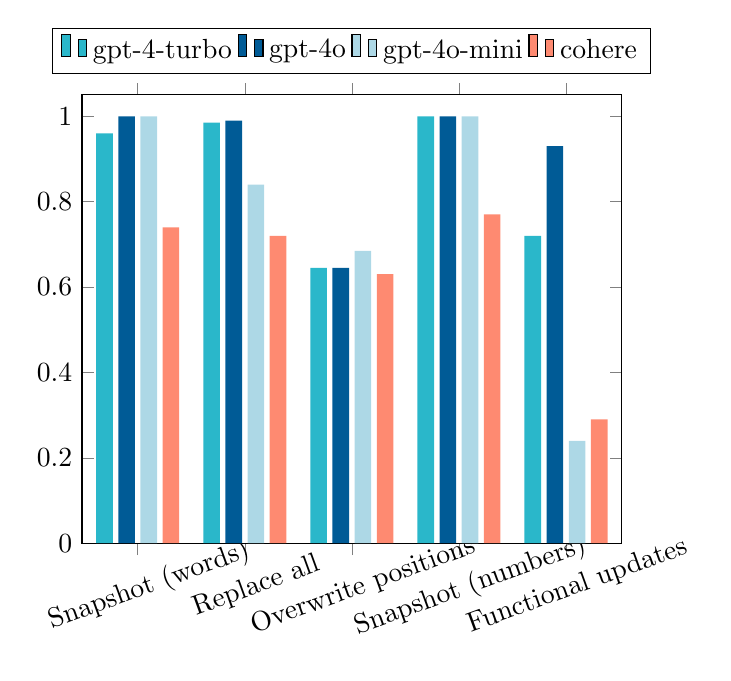
\begin{tikzpicture}
        \begin{axis}[
            ybar,
            bar width=6pt,
            symbolic x coords={Snapshot (words), Replace all, Overwrite positions, Snapshot (numbers), Functional updates},
            xtick=data,
            ymin=0, ymax=1.05,
            legend columns=4,
            legend style={at={(0.5,1.15)}, anchor=north, draw=black},
            enlarge x limits=0.13,
            xticklabel style={rotate=20, anchor=center, yshift=-12pt}
        ]
        
        \addplot[fill={rgb,255:red,42;green,183;blue,202}, draw=none] coordinates {(Snapshot (words),0.96) (Replace all,0.985) (Overwrite positions,0.645) (Snapshot (numbers),1.00) (Functional updates,0.72)};
        \addlegendentry{gpt-4-turbo}
        
        \addplot[fill={rgb,255:red,0;green,91;blue,150}, draw=none] coordinates {(Snapshot (words),1.00) (Replace all,0.99) (Overwrite positions,0.645) (Snapshot (numbers),1.00) (Functional updates,0.93)};
        \addlegendentry{gpt-4o}
        
        \addplot[fill={rgb,255:red,173;green,216;blue,230}, draw=none] coordinates {(Snapshot (words),1.00) (Replace all,0.84) (Overwrite positions,0.685) (Snapshot (numbers),1.00) (Functional updates,0.24)};
        \addlegendentry{gpt-4o-mini}
        
        \addplot[fill={rgb,255:red,254;green,138;blue,113}, draw=none] coordinates {(Snapshot (words),0.74) (Replace all,0.72) (Overwrite positions,0.63) (Snapshot (numbers),0.77) (Functional updates,0.29)};
        \addlegendentry{cohere}
        
        \end{axis}
\end{tikzpicture}}
    \end{subfigure}
    \begin{subfigure}{0.49\columnwidth}
        \resizebox{\textwidth}{!}{    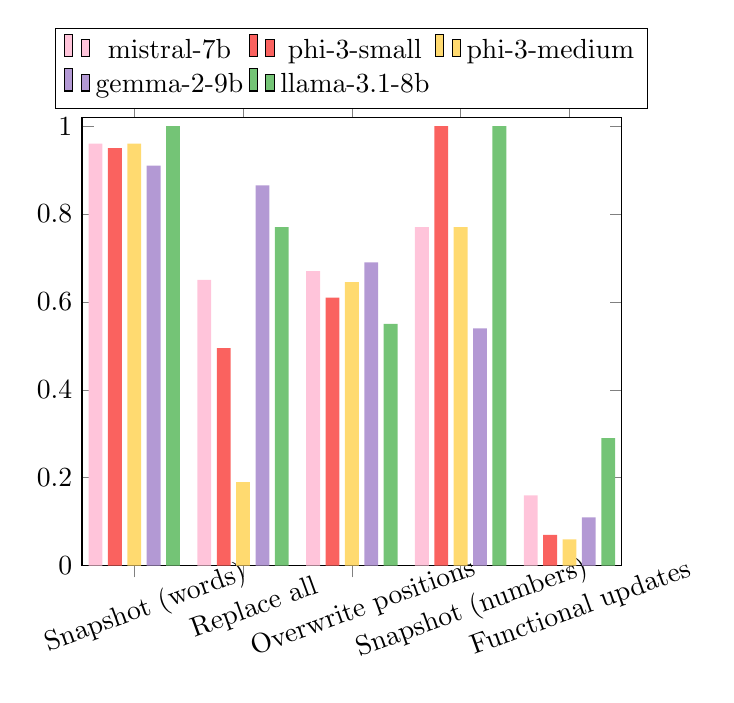
\begin{tikzpicture}
        \begin{axis}[
            ybar,
            bar width=5pt,
            symbolic x coords={Snapshot (words), Replace all, Overwrite positions, Snapshot (numbers), Functional updates},
            xtick=data,
            ymin=0, ymax=1.02,
            legend columns=3,
            legend style={at={(0.5,1.20)}, anchor=north, draw=black},
            enlarge x limits=0.12,
            xticklabel style={rotate=20, anchor=center, yshift=-12pt}
        ]
        
        \addplot[fill={rgb,255:red,255;green,196;blue,218}, draw=none] coordinates {(Snapshot (words),0.96) (Replace all,0.65) (Overwrite positions,0.67) (Snapshot (numbers),0.77) (Functional updates,0.16)};
        \addlegendentry{mistral-7b}
        
        \addplot[fill={rgb,255:red,250;green,98;blue,95}, draw=none] coordinates {(Snapshot (words),0.95) (Replace all,0.495) (Overwrite positions,0.61) (Snapshot (numbers),1.00) (Functional updates,0.07)};
        \addlegendentry{phi-3-small}
        
        \addplot[fill={rgb,255:red,255;green,218;blue,112}, draw=none] coordinates {(Snapshot (words),0.96) (Replace all,0.19) (Overwrite positions,0.645) (Snapshot (numbers),0.77) (Functional updates,0.06)};
        \addlegendentry{phi-3-medium}
        
        \addplot[fill={rgb,255:red,179;green,153;blue,212}, draw=none] coordinates {(Snapshot (words),0.91) (Replace all,0.865) (Overwrite positions,0.69) (Snapshot (numbers),0.54) (Functional updates,0.11)};
        \addlegendentry{gemma-2-9b}
        
        \addplot[fill={rgb,255:red,116;green,196;blue,118}, draw=none] coordinates {(Snapshot (words),1.00) (Replace all,0.77) (Overwrite positions,0.55) (Snapshot (numbers),1.00) (Functional updates,0.29)};
        \addlegendentry{llama-3.1-8b}
        
        \end{axis}
\end{tikzpicture}}
    \end{subfigure}
    \caption{Results for the \textbf{Recall and Edit} tasks.}
    \label{fig:recall}
\end{figure}

\paragraph{Recall and Edit} 
\begin{table}[!h]
    \centering
        \resizebox{0.8\columnwidth}{!}{%
    \begin{tabular}{lllll}
    \toprule
        \textbf{Model} & \textbf{String Search (word)} & \textbf{Snapshot} \\ \hline
gpt-4-turbo    & 1.00 \textcolor{green}{(0.06)} & 1.00 \textcolor{green}{(0.04)} \\ 
gpt-4o         & 1.00 (0.00)                   & 1.00 (0.00)                   \\ 
gpt-4o-mini    & 0.94 \textcolor{red}{(-0.04)}  & 1.00 (0.00)                   \\ 
cohere         & 1.00 (0.00)                   & 1.00 \textcolor{green}{(0.26)} \\ 
mistral-7b     & 1.00 \textcolor{green}{(0.22)} & 0.96 (0.00)                   \\ 
phi-3-small    & 1.00 \textcolor{green}{(0.06)} & 0.99 \textcolor{green}{(0.04)} \\ 
phi-3-medium   & 0.98 \textcolor{red}{(-0.02)}  & 0.87 \textcolor{red}{(-0.09)}  \\ 
gemma-2-9b     & 0.96 \textcolor{red}{(-0.04)}  & 0.96 \textcolor{green}{(0.05)} \\ 
llama-3.1-8b   & 0.98 \textcolor{red}{(-0.02)}  & 1.00 (0.00)                   \\
\bottomrule
    \end{tabular}
    }
    \caption{Ablation study with gibberish context.}
    \label{tab:ablation_gibberish}
\end{table}

Figure \ref{fig:recall} presents the results for the \textbf{Recall and Edit} tasks. While models performed well on basic recall (\textit{Snapshot}), their performance dropped sharply when tasked with making regular edits. A closer analysis of the generated outputs reveals that models struggled with maintaining coherence during edits, often getting trapped in repetitive word loops. For the \textit{Functional Update} task, we deliberately selected simple numerical updates, such as ``Subtract 1 from every number," to ensure the edits were within the models' capabilities. Nevertheless, when comparing performance on \textit{Snapshot (with numbers)} to \textit{Functional Updates}, all models exhibited a steep decline, especially for smaller ones. Analysis of generated outputs revealed that these models frequently deviated from instructions over longer sequences, suggesting difficulties in maintaining consistent rule applications over extended contexts.

Additionally, we conducted a separate ablation study on \textit{Snapshot} and \textit{String Search}. In this study, we replaced meaningful words in the context with gibberish tokens consisting of randomly generated alphabetical characters. As shown in Table \ref{tab:ablation_gibberish}, performance remained largely unchanged, suggesting that semantic meaning was not a significant distractor in these tasks.

\begin{table}
\centering
% \footnotesize
\resizebox{\linewidth}{!}{
\setlength{\tabcolsep}{5pt}
\begin{tabular}[t]{l|ccc}
\toprule
 \makecell[c]{\textbf{Method}} & \makecell[c]{\textbf{Self}\\\textbf{Reflection}} & \makecell[c]{\textbf{Memory}} & \makecell[c]{\textbf{Length}\\\textbf{Generalization}} \\
\midrule
Revision~\cite{DBLP:journals/corr/abs-2408-03314} & \redcross & \greencheck & \redcross \\
Self-Refine~\cite{DBLP:conf/nips/MadaanTGHGW0DPY23} & \greencheck & \greencheck & \redcross \\
Best-of-N~\cite{DBLP:journals/corr/abs-2407-21787} & \redcross & \redcross & \greencheck \\
Beam Search~\cite{ow1988filtered} & \redcross & \redcross & \greencheck \\
Guided Beam Search~\cite{DBLP:conf/nips/XieKZZKHX23} & \greencheck & \redcross & \greencheck \\
\midrule
\textbf{FTTT (ours)} & \greencheck & \greencheck & \greencheck \\
\bottomrule
\end{tabular}
}
% \vspace{-5pt}
\caption{Comparing the advantages and drawbacks of FTTT and related works.}
\label{tab:compare}
% \vspace{-0.5cm}
\end{table}

\begin{table}[!htbp] \centering
  \caption{Human Choices and Predictions About GenAI Choice in the Same Problem: Heterogeneity by Exposure and Attitudes (Pooled)}
\begin{adjustbox}{scale=0.8}
\begin{tabular}{@{\extracolsep{5pt}}lccccc}
% \\[-1.8ex]\hline
% \hline \\[-1.8ex]
\toprule
& \multicolumn{5}{c}{\textit{Dependent variable: Prediction}} \
\cr \cline{2-6}
\\[-1.8ex] & \multicolumn{1}{c}{Heavy User} & \multicolumn{1}{c}{Text-Based LLM User} & \multicolumn{1}{c}{Paid User} & \multicolumn{1}{c}{Agree AI Similar} & \multicolumn{1}{c}{Agree AI Better}  \\
\\[-1.8ex] & (1) & (2) & (3) & (4) & (5) \\
% \hline \\[-1.8ex]
\midrule
 X$\times$Heavy User & -0.056$^{}$ & & & & \\
& (0.052) & & & & \\
 X$\times$Text-Based LLM User & & 0.082$^{**}$ & & & \\
& & (0.040) & & & \\
 X$\times$Paid User & & & -0.001$^{}$ & & \\
& & & (0.072) & & \\
 X$\times$Agree AI Similar & & & & 0.033$^{}$ & \\
& & & & (0.045) & \\
 X$\times$Agree AI Better & & & & & 0.019$^{}$ \\
& & & & & (0.017) \\
 Problem FE & Yes & Yes & Yes & Yes & Yes \\
 X$\times$Problem FE & Yes & Yes & Yes & Yes & Yes \\
 G$\times$Problem FE & Yes & Yes & Yes & Yes & Yes \\
% \hline \\[-1.8ex]
\midrule
 Observations & 2700 & 2700 & 2700 & 2700 & 2700 \\
 % Residual Std. Error & 22.874 & 22.851 & 22.863 & 22.847 & 22.895 \\
% \hline
% \hline \\[-1.8ex]
\bottomrule
\textit{Note:} & \multicolumn{5}{r}{Standard errors are clustered at the problem level. $^{*}$p$<$0.1; $^{**}$p$<$0.05; $^{***}$p$<$0.01} \\
% \multicolumn{6}{r}\textit{} \\
\end{tabular}
\end{adjustbox}
\label{tab:group} \end{table}


\paragraph{Match and Compare}
 As shown in Figure \ref{fig:match}, model performance in the \textbf{Match and Compare} tasks was relatively consistent across different model sizes. Given that counting is a well-known weakness in LLMs, it is unsurprising that all models struggled significantly with the counting task, though GPT models performed slightly better than others. However, models generally succeeded in identifying the duplicates (in \textit{Find duplicates}), and primarily struggled with the counting aspect -- which requires tracking and updating an integer state, a skill that is more similar to stateful processing. This suggests that relying solely on counting-based tests \cite{song2024countingstars} could overly bias the evaluation and fail to capture broader model capabilities. The results also indicate that models exhibit some ability to recognize relative positions and group associations, but their accuracy remains limited (ranging between 0.6-0.8). A closer examination of model generations reveals an overwhelming tendency for the models to produce false positive errors -- models often answer “yes” when the correct answer is “no”, while making very few false negative errors. This means that when the relationship is correct, the models can more reliably identify it. This may stem from a combination of their inherent inclination to agree and the difficulty in recognizing relative comparisons and associations.

% \begin{figure}[h]
%     \centering
%     \includegraphics[width=0.92\columnwidth]{images/difference.png}
%     \caption{Results for \textbf{Spot the Differences }tasks.}
%     \label{fig:difference}
% \end{figure}

\begin{figure}[h]
\centering
\resizebox{0.9\columnwidth}{!}{
 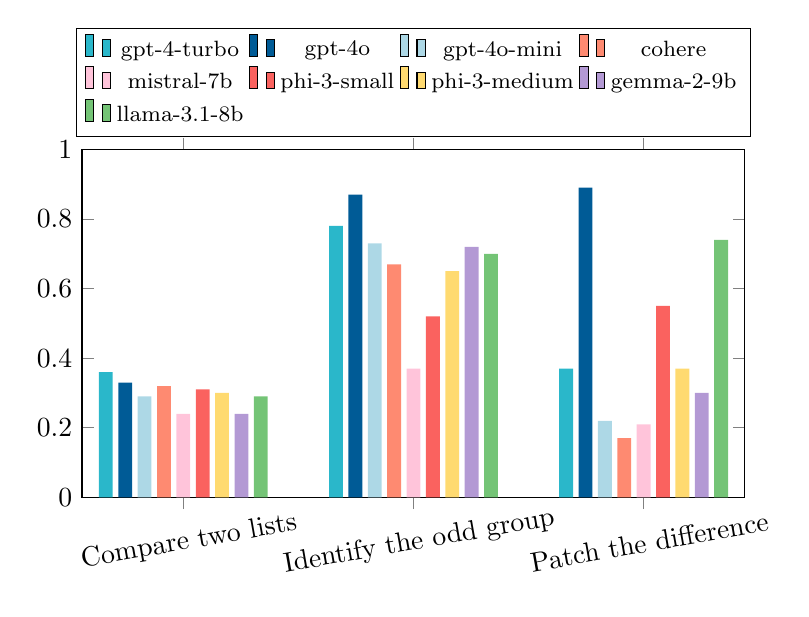
\begin{tikzpicture}
        \begin{axis}[
            ybar,
            bar width=5pt,
            symbolic x coords={Compare two lists, Identify the odd group, Patch the difference},
            xtick=data,
            ymin=0, ymax=1.0,
            legend columns=4,
            legend style={at={(0.5,1.35)}, anchor=north, draw=black, font=\footnotesize},
            enlarge x limits=0.22,
            xticklabel style={rotate=10, anchor=center, yshift=-12pt},
            width=10cm, height=6cm,
        ]
        
        \addplot[fill={rgb,255:red,42;green,183;blue,202}, draw=none] coordinates {(Compare two lists,0.36) (Identify the odd group,0.78) (Patch the difference,0.37)};
        \addlegendentry{gpt-4-turbo}
        
        \addplot[fill={rgb,255:red,0;green,91;blue,150}, draw=none] coordinates {(Compare two lists,0.33) (Identify the odd group,0.87) (Patch the difference,0.89)};
        \addlegendentry{gpt-4o}
        
        \addplot[fill={rgb,255:red,173;green,216;blue,230}, draw=none] coordinates {(Compare two lists,0.29) (Identify the odd group,0.73) (Patch the difference,0.22)};
        \addlegendentry{gpt-4o-mini}
        
        \addplot[fill={rgb,255:red,254;green,138;blue,113}, draw=none] coordinates {(Compare two lists,0.32) (Identify the odd group,0.67) (Patch the difference,0.17)};
        \addlegendentry{cohere}
        
        \addplot[fill={rgb,255:red,255;green,196;blue,218}, draw=none] coordinates {(Compare two lists,0.24) (Identify the odd group,0.37) (Patch the difference,0.21)};
        \addlegendentry{mistral-7b}
        
        \addplot[fill={rgb,255:red,250;green,98;blue,95}, draw=none] coordinates {(Compare two lists,0.31) (Identify the odd group,0.52) (Patch the difference,0.55)};
        \addlegendentry{phi-3-small}
        
        \addplot[fill={rgb,255:red,255;green,218;blue,112}, draw=none] coordinates {(Compare two lists,0.30) (Identify the odd group,0.65) (Patch the difference,0.37)};
        \addlegendentry{phi-3-medium}
        
        \addplot[fill={rgb,255:red,179;green,153;blue,212}, draw=none] coordinates {(Compare two lists,0.24) (Identify the odd group,0.72) (Patch the difference,0.30)};
        \addlegendentry{gemma-2-9b}
        
        \addplot[fill={rgb,255:red,116;green,196;blue,118}, draw=none] coordinates {(Compare two lists,0.29) (Identify the odd group,0.70) (Patch the difference,0.74)};
        \addlegendentry{llama-3.1-8b}
        
        \end{axis}
    \end{tikzpicture}}
    \caption{Results for \textbf{Spot the Differences }tasks.}
    \label{fig:difference}
\end{figure}

\paragraph{Spot the Differences}
As shown in Figure \ref{fig:difference}, performance across all models are poor on \textit{Compare Two Lists}, suggesting inherent difficulties in cross-referencing information across long contexts, even for larger models.  GPT-4o and the LLaMA model significantly outperform the others in the \textit{Identify the Odd Group} task, highlighting a general weakness in detecting contextual differences by the other models. However, an 8B LLaMA model outperforms both equivalently-sized models and even GPT-4 in this task, suggesting that model size alone was not the determining factor. This indicates that architectural differences, training objectives, or specific inductive biases may contribute to improved performance in comparative memory utilization.


\paragraph{Compute on Sets and Lists}
The tasks in this category require models to recognize and process group structures within the context, and performance gradually declines as the complexity of the task increases (see Table \ref{tab:lists}). For instance, in comparing the \textit{Group Membership} task with the \textit{String Search} task, where the former requires identifying which list a word belongs to rather than simply determining its presence, the performance of open-source models drops considerably. Similarly, in comparing the \textit{Group Association} task with the \textit{Group Membership} task, where the former requires determining whether two words belong to the same group, all models exhibit a noticeable decline in performance. The decline becomes even more pronounced when comparing the \textit{ Group Association (alternating)} variant of the task to the standard \textit{Group Association} task. Here, the context involves alternating repeated groups rather than simple group structures, which further challenges the models' abilities to handle partitioned contexts effectively.

An interesting observation was found during the \textit{Iterate} task. In an ablation study, we modified the task to require returning the first words in each list instead of the last words (making it more similar to the \textit{Batch Search} task). The performance sharply declines when models are asked to return the last words, despite their strong information-fetching capabilities. This suggests that, while the models can retrieve information effectively, they struggle to accurately recognize and process partitions within the context.



\begin{table}[t!]
\centering
    \resizebox{0.7\columnwidth}{!}{%

\begin{tabular}{lcc}
\toprule
\textbf{Model} & \textbf{Quantity state} & \textbf{Set state} \\
\midrule
gpt-4-turbo & 0.8 & \textbf{0.80} \\
gpt-4o & \textbf{1.0} & 0.65 \\
gpt-4o-mini & 0.7 & 0.24 \\
cohere & 0.0 & 0.58 \\
mistral-7b & 0.0 & 0.08 \\
phi-3-small & 0.0 & 0.13 \\
phi-3-medium & 0.0 & 0.11 \\
gemma-2-9b & 0.0 & 0.24 \\
llama-3.1-8b & 0.0 & 0.13 \\
\bottomrule
\end{tabular}
}
\caption{Results for \textbf{Stateful Processing} tasks.}
\label{tab:state}
\end{table}
\paragraph{Stateful Processing}

\begin{figure}[t!]
    \centering
    \begin{subfigure}{0.49\columnwidth}
        \resizebox{\textwidth}{!}{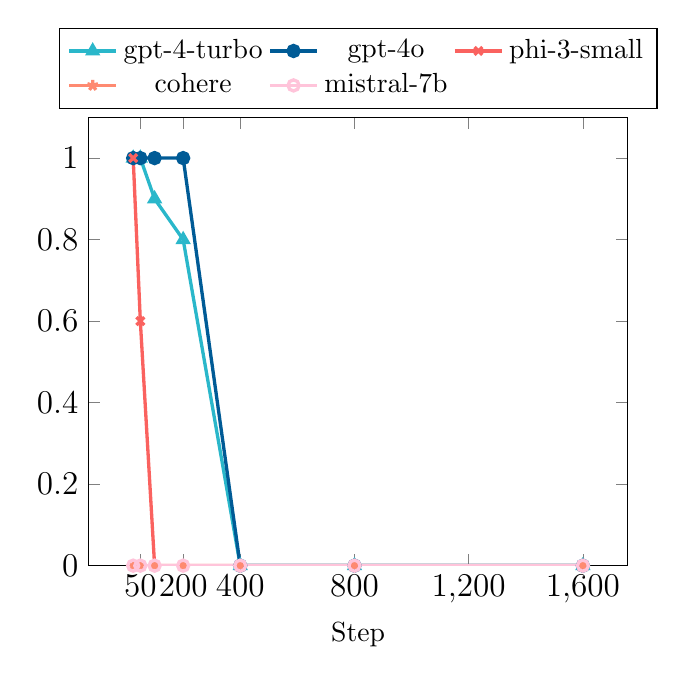
\begin{tikzpicture}
    \begin{axis}[
        xlabel={Step},
        legend style={at={(0.5,1.2)}, anchor=north, cells={align=left}, legend columns=3},
        ymin=0, ymax=1.1,
        xtick={50, 200, 400, 800, 1200, 1600},
        ytick={0,0.2,0.4,0.6,0.8,1.0},
        grid=none,
        tick label style={font=\large}
    ]

    % GPT-4-Turbo
    \addplot[mark=triangle, very thick, color={rgb,255:red,42;green,183;blue,202}] coordinates {
        (25,1.0) (50,1.0) (100,0.9) (200,0.8) (400,0.0) (800,0.0) (1600,0.0)
    };
    \addlegendentry{gpt-4-turbo}

    % GPT-4o
    \addplot[mark=*, very thick, color={rgb,255:red,0;green,91;blue,150}] coordinates {
        (25,1.0) (50,1.0) (100,1.0) (200,1.0) (400,0.0) (800,0.0) (1600,0.0)
    };
    \addlegendentry{gpt-4o}



    % Phi-3-Small
    \addplot[mark=x, very thick, color={rgb,255:red,250;green,98;blue,95}] coordinates {
        (25,1.0) (50,0.6) (100,0.0) (200,0.0) (400,0.0) (800,0.0) (1600,0.0)
    };
    \addlegendentry{phi-3-small}

    % Cohere
    \addplot[mark=star, very thick, color={rgb,255:red,254;green,138;blue,113}] coordinates {
        (25,0.0) (50,0.0) (100,0.0) (200,0.0) (400,0.0) (800,0.0) (1600,0.0)
    };
    \addlegendentry{cohere}

    % Mistral-7B
    \addplot[mark=o, very thick, color={rgb,255:red,255;green,196;blue,218}] coordinates {
        (25,0.0) (50,0.0) (100,0.0) (200,0.0) (400,0.0) (800,0.0) (1600,0.0)
    };
    \addlegendentry{mistral-7b}
    
    \end{axis}
\end{tikzpicture}}
    \end{subfigure}
    \begin{subfigure}{0.49\columnwidth}
        \resizebox{\textwidth}{!}{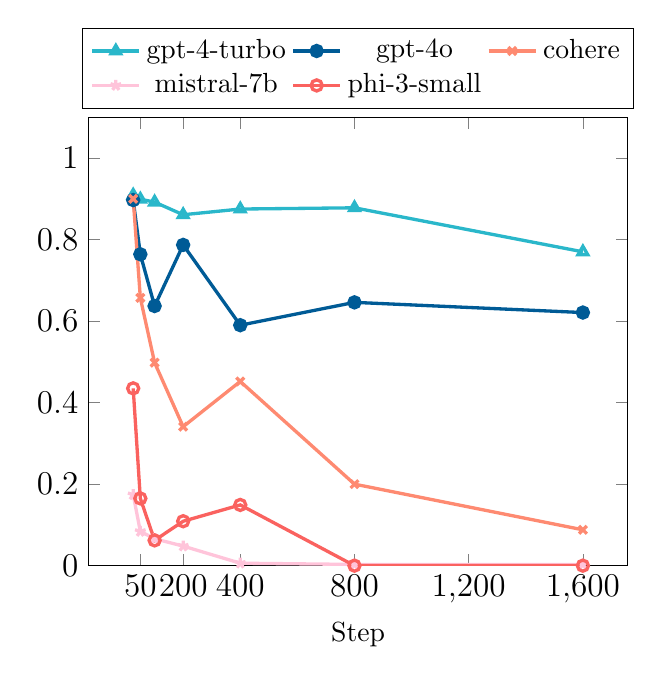
\begin{tikzpicture}
    \begin{axis}[
        xlabel={Step},
        legend style={at={(0.5,1.2)}, anchor=north, cells={align=left}, legend columns=3},
        ymin=0, ymax=1.1,
        xtick={50, 200, 400, 800, 1200, 1600},
        ytick={0,0.2,0.4,0.6,0.8,1.0},
        grid=none,
        tick label style={font=\large}
    ]

    % GPT-4-Turbo
    \addplot[mark=triangle, very thick, color={rgb,255:red,42;green,183;blue,202}] coordinates {
        (25,0.909) (50,0.899) (100,0.892) (200,0.861) (400,0.875) (800,0.878) (1600,0.770)
    };
    \addlegendentry{gpt-4-turbo}

    % GPT-4o
    \addplot[mark=*, very thick, color={rgb,255:red,0;green,91;blue,150}] coordinates {
        (25,0.897) (50,0.764) (100,0.637) (200,0.787) (400,0.590) (800,0.646) (1600,0.621)
    };
    \addlegendentry{gpt-4o}

    % Cohere
    \addplot[mark=x, very thick, color={rgb,255:red,254;green,138;blue,113}] coordinates {
        (25,0.900) (50,0.657) (100,0.498) (200,0.341) (400,0.452) (800,0.200) (1600,0.088)
    };
    \addlegendentry{cohere}

    % Mistral-7B
    \addplot[mark=star, very thick, color={rgb,255:red,255;green,196;blue,218}] coordinates {
        (25,0.174) (50,0.084) (100,0.066) (200,0.048) (400,0.006) (800,0.003) (1600,0.003)
    };
    \addlegendentry{mistral-7b}

    % Phi-3-Small
    \addplot[mark=o, very thick, color={rgb,255:red,250;green,98;blue,95}] coordinates {
        (25,0.435) (50,0.165) (100,0.062) (200,0.109) (400,0.149) (800,0.000) (1600,0.000)
    };
    \addlegendentry{phi-3-small}
    
    \end{axis}
\end{tikzpicture}}
    \end{subfigure}
    \caption{Ablation study on the number of operation steps for the \textbf{quantity state} (left) and\textbf{ set state }(right).}
    \label{fig:ablation_state_step}
\end{figure}



Table \ref{tab:state} presents the results for the \textbf{Stateful Processing} tasks, where performance gaps among models are the most pronounced. The GPT-4(o) models perform well on integer state tracking, while most other models struggle (near zero accuracy). For set state tracking, larger models generally perform better.

We conducted an ablation study to examine how the number of operation steps influences performance of five selected models (Fig. \ref{fig:ablation_state_step}). For quantity state tracking, GPT-4(o) models perform well within fewer than 200 steps but experience a sharp decline in accuracy beyond this threshold. For set state tracking, the performance decline is more gradual. The differences in performance drop between the two tasks can be attributed to the nature of the two tasks. While tracking an integer state might seem simpler than tracking a set, it actually requires the model to maintain and apply every operation sequentially to compute the final value. In contrast, for set state, the fixed size of the set makes more recent operations more relevant to the final state, reducing the need for exhaustive step-by-step tracking. Nevertheless, even in this scenario, all models show a clear inability to handle longer or more complex operation sequences effectively. Interestingly, GPT-4 model outperformed GPT-4o at this task, suggesting potential optimization trade-offs may have affected its ability to manage set-based updates. 

Overall, while larger models like GPT-4(o) exhibit some ability to track state over time, their effectiveness rapidly deteriorates as task complexity increases. Smaller models, in particular, struggle to track operations over time, pointing to significant gaps in their ability to manage and process sequential dependencies critical for state tracking tasks.

\subsection{Results on Composite Tests}

\section{Simple Construction of Projective Compositions}
\label{sec:comp_coord}

It is not clear apriori that projective compositional distributions satisfying Definition \ref{def:proj_comp} ever exist, much less that there is any straightforward way to sample from them.
To explore this, we first restrict attention to perhaps the simplest setting, where the projection functions $\{\Pi_i\}$ are
just coordinate restrictions.
This setting is meant to generalize the intuition we had
in the CLEVR example of Figure~\ref{fig:len_gen},
where different objects were composed in disjoint regions of the image.
We first define the construction of the composed distribution,
and then establish its theoretical properties.








\subsection{Defining the Construction}
Formally, suppose we have a set of distributions
$(p_1, p_2, \ldots, p_k)$ that we wish to compose;
in our running CLEVR example, each $p_i$ is the distribution of images
with a single object at position $i$.
Suppose also we have some reference distribution $p_b$,
which can be arbitrary, but should be thought of as a 
``common background'' to the $p_i$s.
Then, one popular way to construct a composed distribution
is via the \emph{compositional operator} defined below.
(A special case of this construction is used in \citet{du2023reduce}, for example).


\begin{definition}[Composition Operator]
    \label{def:comp_oper}
    Define the \emph{composition operator} $\cC$ acting on an arbitrary set of distributions $(p_b, p_1, p_2, \ldots)$ by
    \begin{align}
    \label{eq:comp_oper}
    \cC[\vec{p}] := \cC[p_b, p_1, p_2, \dots](x) := \frac{1}{Z} p_b(x) \prod_i \frac{p_i(x)}{p_b(x)},
    \end{align}
    where $Z$ is the appropriate normalization constant. We name $\cC[\vec{p}]$ the \emph{composed distribution}, and the score of $\cC[\vec{p}]$ the \emph{compositional score}:
    \begin{align}
    \label{eqn:comp_score}
    &\grad_x \log \cC[\vec{p}](x)  \\
    &= \grad_x \log p_b(x) + \sum_i \left( \grad_x \log p_i(x) - \grad_x \log p_b(x) \right). \notag
    \end{align}
\end{definition}
Notice that if $p_b$ is taken to be the unconditional distribution then this is exactly the Bayes-composition.


\vspace{-0.5em}
\subsection{When does the Composition Operator Work?}
We can always apply the composition operator to any set of distributions,
but when does this actually yield a ``correct'' composition
(according to Definition~\ref{def:proj_comp})?
One special case is when each distribution $p_i$ is
``active'' on a different, non-overlapping set of coordinates.
We formalize this property below
as \emph{Factorized Conditionals} (Definition~\ref{def:factorized}).
The idea is, 
each distribution $p_i$
must have a particular set of ``mask'' coordinates $M_i \subseteq [n]$ which it
samples in a characteristic way,
while independently sampling all other coordinates
from a common background distribution.
If a set of distributions $(p_b, p_1, p_2, \ldots)$ has this
\emph{Factorized Conditional} structure, then 
the composition
operator will produce a projective composition (as we will prove below).



\begin{definition}[Factorized-Conditionals]
\label{def:factorized}

We say a set of distributions $(p_b, p_1, p_2, \dots p_k)$
over $\R^n$
are \emph{Factorized Conditionals} if
there exists a partition of coordinates $[n]$
into disjoint subsets $M_b, M_1, \dots M_k$ such that:
\begin{enumerate}
    \setlength{\itemsep}{1pt}
    \item $(x|_{M_i}, x|_{M_i^c})$ are independent under $p_i$.
    \item $(x|_{M_b}, x|_{M_1}, x|_{M_2}, \dots, x|_{M_k})$
    are mutually independent under $p_b$.
    \item $p_i(x|_{M_i^c}) = p_b(x|_{M_i^c})$.
\end{enumerate}

Equivalently, if we have:
\begin{align}
    p_i(x) &= p_i(x|_{M_i}) p_b(x|_{M_i^c}), \text{ and} \label{eqn:cc-cond}\\
    p_b(x) &= p_b(x|_{M_b}) \prod_{i \in [k]} p_b(x|_{M_i}). \notag
\end{align}
\end{definition}
\vspace{-1em}
Equation~\eqref{eqn:cc-cond} means that each $p_i$
can be sampled by first sampling $x \sim p_b$,
and then overwriting the coordinates of $M_i$
according to some other distribution (which can be specific to distribution $i$).
For instance, the experiment of Figure~\ref{fig:len_gen}
intuitively satisfies this property, since 
each of the conditional distributions could essentially be sampled
by first sampling an empty background image ($p_b$), then ``pasting''
a random object in the appropriate location (corresponding to pixels $M_i$).
If a set of distributions obey this Factorized Conditional structure,
then we can prove that the composition operator $\cC$
yields a correct projective composition,
and reverse-diffusion correctly samples from it.
Below, let $N_t$ denote the noise operator of the
diffusion process\footnote{Our results are agnostic to the specific diffusion noise-schedule and scaling used.} at time $t$.

\begin{theorem}[Correctness of Composition]
\label{lem:compose}
Suppose a set of distributions $(p_b, p_1, p_2, \dots p_k)$
satisfy Definition~\ref{def:factorized},
with corresponding masks $\{M_i\}_i$.
Consider running the reverse-diffusion SDE 
using the following compositional scores at each time $t$:
\begin{align}
s_t(x_t) &:= \grad_x \log \cC[p_b^t, p_1^t, p_2^t, \ldots](x_t),
\end{align}
where $p_i^t := N_t[p_i]$ are the noisy distributions.
Then, the distribution of the generated sample $x_0$ at time $t=0$ is:
\begin{align}
\label{eqn:p_hat}
\hat{p}(x) := p_b(x|_{M_b}) \prod_i p_i(x|_{M_i}).
\end{align}
In particular,
$\hat{p}(x|_{M_i}) = p_i(x|_{M_i})$ for all $i$,
and so
$\hat{p}$ is a projective composition
with respect to projections $\{\Pi_i(x) := x|_{M_i}\}_i$,
per Definition \ref{def:proj_comp}.
\end{theorem}




Unpacking this, Line \ref{eqn:p_hat} says that the final generated distribution
$\hat{p}(x)$ can be sampled by
first sampling
the coordinates $M_b$ according to $p_b$ (marginally),
then independently sampling 
coordinates $M_i$ according to $p_i$ (marginally) for each $i$.
Similarly, by assumption, $p_i(x)$ can be sampled by first sampling the coordinates $M_i$ in some specific way, and then independently sampling the remaining coordinates according to $p_b$. Therefore Theorem \ref{lem:compose} says that $\hat{p}(x)$ samples the coordinates \emph{$M_i$ exactly as they would be sampled by $p_i$}, for each $i$ we wish to compose. 

\begin{proof}(Sketch) \small
Since $\vec{p}$ satisfies Definition \ref{def:factorized}, we have
\begin{align*}
&\cC[\vec{p}](x) := p_b(x) \prod_i \frac{p_i(x)}{p_b(x)} \notag 
= p_b(x) \prod_i \frac{p_b(x_t|_{M_i^c}) p_i(x|_{M_i})}{p_b(x|_{M_i^c})p_b(x|_{M_i})} \notag \\
&= p_b(x) \prod_i \frac{p_i(x|_{M_i})}{p_b(x|_{M_i})} \notag 
= p_b(x|_{M_b}) \prod_i p_i(x_t|_{M_i}) := \hat{p}(x).
\end{align*}
The sampling guarantee follows from the commutativity of composition with the diffusion noising process, i.e. $\cC[\vec{p^t}]= N_t[\cC[\vec{p}]]$. 
The complete proof is in Appendix \ref{app:compose_pf}.
\end{proof}

\begin{remark}
In fact, Theorem~\ref{lem:compose} still holds under any orthogonal transformation of the variables,
because the diffusion noise process commutes with orthogonal transforms.
We formalize this as Lemma~\ref{lem:orthogonal_sampling}.
\end{remark}

\begin{remark}
Compositionality is often thought of in terms of orthogonality between scores.
Definition \ref{def:factorized} implies orthogonality between the score differences that appear in the composed score \eqref{eqn:comp_score}:
$\grad_x \log p_i^t(x_t) - \grad_x \log p_b^t(x_t),$
but the former condition is strictly stronger
(c.f. Appendix \ref{app:score_orthog}).
\end{remark}

\begin{remark}
Notice that the composition operator $\cC$
can be applied to a set of Factorized Conditional
distributions
without knowing the coordinate partition $\{M_i\}$.
That is, we can compose distributions and compute scores
without knowing apriori exactly ``how'' these distributions are supposed to compose
(i.e. which coordinates $p_i$ is active on).
This is already somewhat remarkable, and we will see a much
stronger version of this property in the next section.
\end{remark}

\textbf{Importance of background.}
Our derivations highlight the crucial role of the background
distribution $p_b$ for the composition operator  
(Definition~\ref{def:comp_oper}).
While prior works have taken $p_b$ to be an unconditional distribution and the $p_i$'s its associated conditionals,
our results suggest this is not always the optimal choice -- in particular,
it may not satisfy a Factorized Conditional structure (Definition~\ref{def:factorized}). Figure~\ref{fig:len_gen_monster} demonstrates this empirically: settings (a) and (b) attempt to compose the same distributions using different backgrounds -- empty (a) or unconditional (b) -- with very different results.

\subsection{Approximate Factorized Conditionals in CLEVR.}
\label{sec:clevr-details}

In \cref{fig:len_gen_monster} we explore compositional length-generalization (or lack thereof) in three different setting, two of which (\cref{fig:len_gen_monster}a and \ref{fig:len_gen_monster}c) approximately satisfy \cref{def:factorized}. In this section we explicitly describe how our definition of Factorized Conditionals approximately captures the CLEVR settings of Figures \ref{fig:len_gen_monster}a and \ref{fig:len_gen_monster}c. The setting of \ref{fig:len_gen_monster}b does not satisfy our conditions, as discussed in \cref{sec:problematic-compositions}.

\textbf{Single object distributions with empty background.}
This is the setting of both \cref{fig:len_gen} and \cref{fig:len_gen_monster}a.
The background distribution $p_b$ 
over $n$ pixels is images of an empty scene with no objects.
For each $i \in \{1,\ldots,L\}$ (where $L=4$ in \cref{fig:len_gen} and $L=9$ in \cref{fig:len_gen_monster}a), define the set $M_i \subset [n]$ 
as the set of pixel indices surrounding location $i$.
($M_i$ should be thought of as a ``mask'' that
that masks out objects at location $i$).
Let $M_b := (\cup_i M_i)^c$ be the remaining
pixels in the image.
Then, we claim the distributions $(p_b, p_1, \ldots, p_L)$
form approximately
Factorized Conditionals, with corresponding
coordinate partition $\{M_i\}$.
This is essentially because each distribution $p_i$
matches the background $p_b$ on all pixels except those surrounding
location $i$ (further detail in Appendix~\ref{app:clevr-details}).
Note, however, that the conditions of Definition~\ref{def:factorized}
do not \emph{exactly} hold in the experiment of Figure~\ref{fig:len_gen} -- there is still some dependence between
the masks $M_i$, since objects can cast shadows or even occlude each other.
Empirically, these deviations 
have greater impact
when composing many objects, as seen in \cref{fig:len_gen_monster}a.


\textbf{Bayes composition with cluttered distributions.}
In \cref{fig:len_gen_monster}c we replicate CLEVR experiments in  \citet{du2023reduce, liu2022compositional} where the images contain many objects (1-5) and the conditions label the location of one randomly-chosen object. It turns out the unconditional together with the conditionals can approximately act as Factorized Conditionals in ``cluttered'' settings like this one. The intuition is that if the conditional distributions each contain one specific object plus many independently sampled random objects (``clutter''), then the unconditional distribution \emph{almost} looks like independently sampled random objects, which together with the conditionals \emph{would} satisfy Definition \ref{def:factorized} (further discussion in Appendix \ref{app:clevr-details} and \ref{app:bayes_connect}). This helps to explain the length-generalization observed in \citet{liu2022compositional} and verified in our experiments (\cref{fig:len_gen_monster}c).







\section{Projective Composition in Feature Space}
\label{sec:comp_feature}

\begin{figure}
    \centering
    \includegraphics[width=1.0\linewidth]{figures/feat-space-vis.png}
    \caption{A commutative diagram illustrating Theorem~\ref{lem:transform_comp}.
    Performing composition in pixel space is equivalent 
    to encoding into a feature space ($\cA$),
    composing there,
    and decoding back
    to pixel space ($\cA^{-1}$).
    }
    \label{fig:feat-space-vis}
\end{figure}

So far we have focused on the setting where the projection functions $\Pi_i$ are simply projections onto coordinate subsets $M_i$ in the native space (e.g. pixel space).
This covers simple examples like Figure~\ref{fig:len_gen} but does not include more realistic situations such as Figure~\ref{fig:style-content},
where the properties to be composed are more abstract.
For example a property like ``oil painting'' does not correspond to projection
onto a specific subset of pixels in an image.
However, we may hope that there exists some conceptual feature space
in which ``oil painting'' does correspond to a particular subset of variables.
In this section, we extend our results to the case where the composition occurs in some conceptual feature space, and each distribution to be composed
corresponds to some particular subset of \emph{features}.


Our main result is a featurized analogue of Theorem~\ref{lem:compose}:
if there exists \emph{any} invertible transform $\cA$
mapping into a feature space
where Definition \ref{def:factorized} holds,
then the composition operator (Definition~\ref{def:comp_oper})
yields a projective composition in this feature space, as shown in Figure~\ref{fig:feat-space-vis}.

\begin{theorem}[Feature-space Composition]
\label{lem:transform_comp}
Given distributions $\vec{p} := (p_b, p_1, p_2, \dots p_k)$,
suppose there exists a diffeomorphism $\cA: \R^n \to \R^n$
such that
$(\cA \sharp p_b, \cA \sharp p_1, \dots \cA \sharp p_k)$
satisfy Definition~\ref{def:factorized},
with corresponding partition $M_i \subseteq [n]$.
Then, the composition $\hat{p} := \cC[\vec{p}]$ satisfies:
\begin{align}
\label{eqn:p_hat_A}
\cA \sharp \hat{p}(z)
\equiv
(\cA \sharp p_b (z))|_{M_b} \prod_{i=1}^k (\cA \sharp p_i(z))|_{M_i}.
\end{align}
Therefore, $\hat{p}$
is a projective composition of $\vec{p}$ w.r.t. projection functions
$\{\Pi_i(x) := \cA(x)|_{M_i}\}$.
\end{theorem}
This theorem is remarkable because it means we can
compose distributions $(p_b, p_1, p_2, \dots)$ in the base space,
and this composition will ``work correctly'' in the feature space
automatically (Equation~\ref{eqn:p_hat_A}),
without us ever needing to compute or even know the feature transform $\cA$
explicitly.



Theorem~\ref{lem:transform_comp} may apriori seem too strong
to be true, since it somehow holds for all feature spaces $\cA$
simultaneously.
The key observation underlying Theorem~\ref{lem:transform_comp} 
is that the composition operator $\cC$ behaves
well under reparameterization.
\begin{lemma}[Reparameterization Equivariance]
\label{lem:reparam}
The composition operator of Definition~\ref{def:comp_oper}
is reparameterization-equivariant. That is,
for all diffeomorphisms $\cA: \R^n \to \R^n$
and all tuples of distributions $\vec{p} = (p_b, p_1, p_2, \dots, p_k)$,
\begin{align}
 \cC[ \cA \sharp \vec{p}] =  \cA \sharp \cC[\vec{p}].
\end{align}
\end{lemma}
\arxiv{\footnote{
For example (separate from our goals in this paper):
Classifier-Free-Guidance can be seen as an instance of the composition operator.
Thus, Lemma~\ref{lem:reparam} implies that performing CFG
in latent space is \emph{equivalent} to CFG in pixel-space,
assuming accurate score-models in both cases.}}
\arxiv{This lemma is potentially of independent interest:
reparametrization-equivariance
is a very strong property which is typically not satisfied by
standard operations between probability distributions---
for example, the ``simple product'' $p_1(x)p_2(x)$ does not satisfy it---
so it is mathematically notable that the composition operator 
has this structure.
Lemma~\ref{lem:reparam} and Theorem~\ref{lem:transform_comp}
are proved in Appendix \ref{app:param-indep}.}

This lemma is potentially of independent interest:
equivariance distinguishes the composition operator
from many other common operators
(e.g. the simple product).
Lemma ~\ref{lem:reparam} and Theorem~\ref{lem:transform_comp}
are proved in Appendix \ref{app:param-indep}.

\section{Sampling from Compositions.}
The feature-space Theorem~\ref{lem:transform_comp} is weaker than Theorem~\ref{lem:compose}
in one important way: it does not provide a sampling algorithm.
That is, Theorem~\ref{lem:transform_comp} guarantees that $\hat{p} := \cC[\vec{p}]$
is a projective composition, but does not guarantee that reverse-diffusion
is a valid sampling method.

There is one special case where diffusion sampling \emph{is} guaranteed to work, namely, for orthogonal transforms (which can seen as a straightforward extension of the coordinate-aligned case of \cref{lem:compose}):
\begin{lemma}[Orthogonal transform enables diffusion sampling]
\label{lem:orthogonal_sampling}
If the assumptions of Lemma \ref{lem:transform_comp} hold for $\cA(x) = Ax$, where $A$ is an orthogonal matrix, then running a reverse diffusion sampler with scores $s_t = \grad_x \log \cC[\vec{p}^t]$ generates the composed distribution $\hat{p} = \cC[\vec{p}]$ satisfying \eqref{eqn:p_hat_A}.
\end{lemma}
The proof is given in \cref{app:orthog_sample_pf}.

However, for general invertible transforms, we have no such sampling guarantees.
Part of this is inherent: in the feature-space setting, the 
diffusion noise operator $N_t$ no longer commutes
with the composition operator $\cC$ in general,
 so scores of the noisy composed 
distribution $N_t[\cC[\vec{p}]]$
cannot be computed from scores
of the noisy base distributions $N_t[\vec{p}]$.
Nevertheless, one may hope to sample from the distribution $\hat{p}$
using other samplers besides diffusion, 
such as annealed Langevin Dynamics
or
Predictor-Corrector methods \citep{song2020score}.
We find that the situation is surprisingly subtle:
composition $\cC$ produces distributions which
are in some cases easy to sample (e.g. with diffusion),
yet in other cases apparently hard to sample.
For example, in the
setting of Figure~\ref{fig:clevr_color_comp}, 
our Theorem~\ref{lem:transform_comp} implies
that all pairs of colors should compose equally well
at time $t=0$, since there exist diffeomorphisms
(indeed, linear transforms) between different colors.
However, as we saw,
the diffusion sampler
fails to sample from compositions 
of non-orthogonal colors--- and 
empirically, even more sophisticated
samplers such as Predictor-Correctors
also fail in this setting.
At first glance, it may seem odd that
composed distributions are so hard to sample,
when their constituent distributions are relatively easy to sample.
One possible reason for this below is that the composition operator has extremely poor Lipchitz constant,
so it is possible for a set of distributions $\vec{p}$ to ``vary smoothly''
(e.g. diffusing over time) while their composition $\cC[\vec{p}]$
changes abruptly.
We formalize this in \cref{lem:lipschitz} (further discussion and proof in Appendix \ref{app:lipschitz}).
\begin{lemma}[Composition Non-Smoothness]
\label{lem:lipschitz}
For any set of distributions $\{p_b, p_1, p_2, \dots, p_k\}$,
and any noise scale $t := \sigma$,
define the noisy distributions 
$p_i^t := N_{t}[p_i]$,
and let $q^t$ denote the composed distribution at time $t$: $q^t := \cC[\vec{p}^t]$. Then, for any choice of $\tau > 0$,
there exist distributions $\{p_b, p_1, \dots p_k\}$ over $\R^n$
such that
\begin{enumerate}
    \setlength{\itemsep}{0pt}
    \item For all $i$, the annealing path of $p_i$ is 
    $\cO(1)$-Lipshitz:
    $\forall t, t': W_2(p_i^{t}, p_i^{t'}) \leq \cO(1) |t - t'|$.
    \item The annealing path of $q$ has Lipshitz constant
    at least $\Omega(\tau^{-1})$:
    $\exists t, t': W_2(q^{t}, q^{t'}) \geq \frac{|t - t'|}{2\tau}.$
\end{enumerate}
\end{lemma}




The composite tests significantly challenge the models by combining multiple atomic capabilities into a single test. In the \textit{Processing Data Blocks} task, the context is fixed at 4k tokens, while for the \textit{Theory of Mind} task, the number of operation steps is set to 100. As shown in Table \ref{tab:comp}, model performance on both tasks are generally low, showing a broad inability to handle the more complex scenarios. Performance across all models drop substantially on composite tasks compared to their performance on individual capability tasks, such as search, recall, and group processing. 

Interestingly, some smaller models, like Mistral and Phi-3-small, exhibit slightly better performance on the \textit{Theory of Mind} task than on the set state tracking task. This anomaly likely stems from their already weak state tracking ability, which limits their performance across both tasks. Additionally, these models tend to generate longer answers in the set state task which reduces the set overlap.

Notably, even the most capable models, such as GPT-4-turbo and GPT-4o, struggle, showing that scaling model size alone is not enough for solving these composite tasks. Additionally, the variation in performance among smaller models suggests that their limitations stem not only from size but also from underlying architectural or training differences. This indicates that smaller models require more targeted care to bridge the gap in effective memory use.



\section{Downstream Tasks}
\label{sec:downstream_tasks}
In this section, we show the effectiveness of the Wizard-of-Shopping dataset by applying it to two downstream tasks: Conversational Query Generation (CQG) and Conversational Product Ranking (CPR). For both tasks, we divided the \textit{WoS} conversations into 3,000 for training, 300 for validation, and 300 for testing, with each split containing an equal number of dialogues from the three domains. More details are available in Appendix \ref{sec:detailed_downstream_tasks}.

\subsection{Conversational Query Generation (CQG)}

Real product search conversations are likely to be verbose and redundant for the purpose of product ranking.  
Similar to the conversational search~\cite{yu2020few,vakulenko2021question,chen-etal-2022-reinforced,wu2022conqrr} where a reformulation model is used to generate a more informative query from the dialogue history, we address \textit{conversational query generation} (CQG) for product search. 
CQG aims to extract essential information such as the product category under discussion, desired features, undesired features, and optional product preferences from the customer. This extracted information can then be used as a query for a product search engine. And in fact, this is a reverse task of the LLM verbalization where we extract user preferences from the shopping dialogues. Similar to Dialogue State Tracking~\cite{lu2023dialgen}, CQG is helpful in tracing the interest of customers during the conversation. 
%can be extracted for product ranking and DST while the conversation is in progress.
%As the reverse task of the LLM verbalization, the CQG task condenses a long shopping conversation into a structured form that encodes the most essential information about conversational product search. %\shervin{What is the purpose of the task? what is it used for?} 
As \citet{bi2019conversational} suggests, utilizing positive and negative product features are crucial for training a conversational product ranking model. We train a conversational query generator on the \textit{WoS} data to extract the product category and the customer-preferred product features:
%\begin{equation*}
%\vspace{-1em}
\begin{equation}\label{eq:cqg}  \small
    [PC, Wanted, Unwanted, Optional] \gets CQG(Dialogue)
\end{equation}
\vspace{-2em}
%\hl{Jason: is this input same to preference?} % Xiangci: Yes.



\subsubsection{Approaches} \label{sec:conversational_query_generation_approaches}

\paragraph{Baseline.} As stated in \S\ref{sec:related_work}, to the best of our knowledge, \textit{WoS} is the only CPS dataset that can be used for training downstream tasks. Therefore as a simple baseline, we directly use the full conversation history as the predicted query.
%\vspace{-0.5em}
\paragraph{Dialogue --> Query (D2Q).} We use a seq2seq model, Longformer Encoder-Decoder \citep[LED;][]{beltagy2020longformer} fine-tuned on our \textit{WoS} dataset to predict the product category and the \textit{wanted}, \textit{unwanted} and \textit{optional} product features, given the full conversation history.

\paragraph{D2Q (GPT-4).} For reference of LLM performance, we few-shot prompt OpenAI gpt-4-turbo-2024-04-09 with the same inputs and outputs as D2Q.
%\paragraph{Utterance-level.} We assume that each utterance between the seller and customer encodes one or more product features. We use a seq2seq model to extract product features from each utterance, and concatenate the features to be the final query.

% \begin{table}[t]  \small
% \centering
% \setlength{\tabcolsep}{4pt}
% \begin{tabular}{lllllll}
% \hline
% \textbf{Approach} & \textbf{Features} & \textbf{F1} & \textbf{R-1} & \textbf{R-2} & \textbf{R-L}\\ \hline
% Baseline & + & 0 & 0.056 & 0.020 & 0.048 \\ 
% Baseline & +/-/? & 0.008 & 0.137 & 0.047 & 0.087  \\  \hline 
% %Utterance & BART & + & 0.698 & 0.592 & 0.482 & 0.562 \\ 
% %Utterance & BART & +/-/? & 0.656 & 0.664 & 0.489 & 0.592 \\  \hline
% %Utterance & LED & + & 0.704 & 0.610 & 0.509 & 0.578 \\ 
% %Utterance & LED & +/-/? & 0.748 & 0.720 & 0.561 & 0.657 \\  \hline
% D2Q & + & 0.834 & 0.899 & 0.822 & 0.873 \\ 
% D2Q & +/-/? & 0.873 & 0.900 & 0.768 & 0.840 \\  \hline
% \end{tabular}
% \vspace{-0.5em}
% \caption{Conversational Query Generation performance at the final turn measured by exact-F1, ROUGE-1, -2, and -L. We report the performance of only using the desired features (+) for downstream ranking, as well as using all features (wanted (+), unwanted (-), and optional (?)).}
% \label{tab:conversational_query_generation}
% \vspace{-2em}
% \end{table}

\begin{table}[t]  \small
\centering
\setlength{\tabcolsep}{4pt}
\begin{tabular}{llllll}
\hline
\textbf{Approach} & \textbf{F1} & \textbf{R-1} & \textbf{R-2} & \textbf{R-L}\\ \hline
%Baseline & 0 & 0.056 & 0.020 & 0.048 \\ 
Baseline & 0.008 & 0.137 & 0.047 & 0.087  \\  \hline  
%Utterance & BART & + & 0.698 & 0.592 & 0.482 & 0.562 \\ 
%Utterance & BART & +/-/? & 0.656 & 0.664 & 0.489 & 0.592 \\  \hline
%Utterance & LED & + & 0.704 & 0.610 & 0.509 & 0.578 \\ 
%Utterance & LED & +/-/? & 0.748 & 0.720 & 0.561 & 0.657 \\  \hline
D2Q & 0.834 & 0.899 & 0.822 & 0.873 \\ \hline
D2Q (GPT-4) & 0.553 & 0.793 & 0.628 & 0.734 \\ \hline
%D2Q & +/-/? & 0.873 & 0.900 & 0.768 & 0.840 \\  \hline
\end{tabular}
\vspace{-0.5em}
\caption{Conversational Query Generation performance at the final turn measured by exact-F1, ROUGE-1, -2, and -L.}
\label{tab:conversational_query_generation}
\vspace{-2em}
\end{table}

\subsubsection{Experimental Results}
Table \ref{tab:conversational_query_generation} shows the performance of the CQG task.
%We report results on two settings: \textit{wanted} feature-only setups concatenate the product category and \textit{wanted} features and all feature setups concatenate all features as defined in Eq.~\ref{eq:cqg}. 
As expected, the weak baseline using conversation history performs poorly, while our fine-tuned query generator performs much better. %Additionally, we observe that predicting product features utterance-by-utterance instead underperforms using the full conversation (\S\ref{sec:detailed_conversational_query_generation} \& Table \ref{tab:detailed_conversational_query_generation}), which is consistent with prior work of reformulating conversations into queries \cite{yu2020few, wu2022conqrr}. 
Although GPT-4's performance is slightly underestimated because few-shot demonstration examples do not show every edge case, D2Q by \textit{WoS}-finetuned LED shows its superiority of both performance and cost in terms of both latency and price over GPT-4 as an example of LLM.
%When comparing the utterance-level approaches, LED outperforms BART, since the training data for BART is slightly smaller than LED's. This is because we have to discard the input augmented conversation history that is too long for BART's maximum context window (1024 tokens). Also, the LED-based utterance level approach under-performs the conversation level approach, presumably because integrating the results from multiple inferences passes is more error-prone. 

\subsection{Conversational Product Ranking (CPR)}
As the core component of CPS, CPR directly ranks the candidate products given the shopping conversation. We index or embed each product's title and concatenate their aspect-value pairs according to the following approaches:

\subsubsection{Approaches}%\zhiyu{Define what is indexed for each document/product. Title ? Description ?}

\paragraph{Baseline} %Similar to the CQG task, we assume there is no conversational data available for training a ranker. Therefore, w
We directly feed the full conversation history as the query to a BM25 ranker.

%\paragraph{Dialogue --> Product (D2P)} We directly embed the full conversation history to a dense ranker to rank the candidate products, i.e. \textit{Products = Ranker(Dialogue)}. %\zhiyu{related to my previous comments. If products are ranked by Relevance = Ranker(dialogue, product\_info), what is product\_info here?}
\vspace{-0.5em}
\paragraph{Dialogue --> Query --> Product (D2Q2P)} We use D2Q setting in \S\ref{sec:conversational_query_generation_approaches} to generate queries given the full conversation history and apply the queries to a ranker, i.e. \textit{Products = Ranker(CQG(Dialogue))}. We experiment with both a sparse ranker, BM25, and a dense ranker \citep[fine-tuned RoBERTa;][]{liu2019roberta}.

\paragraph{D2Q2P (GPT-4)} We use D2Q (GPT-4) setting in \S\ref{sec:conversational_query_generation_approaches} and feed the predicted query to a BM25 ranker.

\begin{table}[t]  \small
\centering
\setlength{\tabcolsep}{2pt} % Default value: 6pt
\renewcommand{\arraystretch}{1.0} % Default value: 1
\begin{tabular}{llllllll}
\hline
\textbf{Approach} & \textbf{Ranker} & \textbf{MRR} & \textbf{H@1} & \textbf{H@10} & \textbf{H@100}\\ \hline
Baseline & BM25& 0.162 & 0.107 & 0.203 & 0.587 \\ \hline \hline
%D2P & - & longformer & 0.201 & 0.143  & 0.247 & 0.620 \\ \hline
%Utterance & BART & BM25& 0.629 & 0.540  & 0.733 & 0.900 \\
%Utterance & BART & Roberta& 0.217 & 0.163 & 0.270 & 0.477\\ \hline
%Utterance & LED & BM25& 0.667 & 0.593 & 0.740 & 0.900 \\
%Utterance & LED & Roberta& 0.207 & 0.163 & 0.250 & 0.460 \\ \hline
D2Q2P & BM25& \textbf{0.838} & \textbf{0.767}  & \textbf{0.927} & \textbf{0.993} \\
D2Q2P & Roberta & 0.675 & 0.583  & 0.780 & 0.937 \\ \hline
D2Q2P (GPT-4) & BM25 & 0.763 & 0.680 & 0.903 & 0.903 \\ \hline 

\end{tabular}
\vspace{-0.5em}
\caption{Downstream CPR performance at the final turn.}
\label{tab:ranker}
\vspace{-2em}
\end{table}

\subsubsection{Experimental Results}
Table \ref{tab:ranker} shows the mean reciprocal rank (MRR) and Hit$@k$ of all methods. 
%We observe that the D2P approach only slightly outperforms the baseline approach without training. We suspect that our DPR-Longformer is still under-fitted given 3000 conversations as the training set. On the contrary, by leveraging the query generators trained on our collected conversations, the ranking performance is greatly improved. 
%Similar to the trend observed in the conversational query generation task, the conversation-level approach outperforms the utterance-level approach that integrates multiple passes of inference outputs. 
Similar to the trend observed for CQG, our D2Q2P approach significantly outperforms the baseline and GPT-4. Interestingly, the sparse BM25 ranker greatly outperforms the dense RoBERTa-based ranker. This is because the product representations include feature names that are lexically similar to the gold queries. Consequently, BM25 exhibits a strong performance in this ranking task. Moreover, the dense ranker may be under-fitted. The query generators and dense rankers fine-tuned on our \textit{WoS} dataset significantly outperform the baseline that is not trained on our dataset.


\section{Conclusions}
We propose a method, \method, to automatically generate target-oriented shopping conversations without any human annotations. 
% Unlike prior work that learns various user or item representations, \method adds a conversation layer on top of the traditional product search to achieve CPS. 
We leverage decision tree to explore the vast product search space, and construct a dialogue plan that minimizes the number of search steps required to retrieve a relevant product.
%We then successfully compute a dialogue plan that is suitable for feeding into LLMs as prompts, and that guarantees the success of product search with the fewest product features to be clarified.
The resulting corpus (\textit{WoS}), generated using single-pass approach with GPT-4, not only achieved highly natural (4.2/5.0) and coherent (4.7/5.0) ratings from human annotators, but also showed substantial improvements when applied to two downstream tasks. By releasing our dataset and approach, we hope to expedite the research and development of intelligent CPS systems in future.

%We further improve the naturalness of our generated conversations through carefully curated prompts, dynamically listing example product values and leveraging the internal knowledge of the LLMs. We use \method's single pass generation technique with GPT-4 to create and release the \textit{Wizard-of-Shopping} (\textit{WoS}) dataset. Human evaluation shows it is sufficiently natural. Finally, we utilize \textit{WoS} to fine-tune models for downstream CQG and CPR tasks, and find that they significantly outperform baselines not trained on our dialogue dataset. %without using our dataset for training. Therefore, we conclude that our collected CPS dataset can effectively improve the downstream tasks.


\section*{Limitations}
%\subsection{Limitations}
Despite the demonstrated potential of our \method approach and the \textit{WoS} dataset, there are still some limitations that we leave for future work. %\jason{maybe we should work on summarizing all these restrictions. We definitely should discuss limitations, but not sure it is the best place to enumerate all at the last paragraph of our paper. Maybe create a separate section called limitation on section 6?} 
%First, the diversity of our conversations is still insufficient. We find that high-performing LLMs including GPT-4 are not sensitive to instructions regarding \textit{customer persona} (e.g., customer patience, expertise level). Thus, there is no distinction between multiple customers across conversations other than search behavior preferences. 
%Next, \textit{WoS} conversations are all target-oriented with a similar conversation flow -- starting with stating the target product category, identifying the product feature requirements, and finally recommending a qualifying product to the customer. Consequently, 
First, \method does not consider more complicated shopping behavior such as comparison among similar products~\cite{vedula2022matters}. %, or allowing customers to change their mind and roll back to a previous state. 
In the future, we could extend the ability of \method and allow customers to choose a similar product in the search results for comparison with assistance from a LLM agent. 
Second, the quality of \textit{WoS} conversations relies on the quality of the product catalog. Since noise in the product catalog can directly propagate to the generated conversations. Methods proposed to curate and clean the product catalog~\cite{ghani2006text,yang2022mave,vedula2022matters} could be applied to further clean a product catalog. %Moreover, the vocabulary size \jason{this seems redundant. in different places you already talk about the OOV problem} of the product features may directly affect the diversity of the conversation, as well as the feasibility of using the interactive system as a virtual shopping assistant. 
Finally, since the decision tree treats every product aspect and value as a categorical label, the semantics of product features are under-utilized. Future work may further leverage the zero-shot ability of LLMs to mine the semantics of the product aspects, so that similar product features may be merged to produce a more natural and efficient dialogue plan.

\section*{Ethical Statements}
The potential risk of our work could be biased simulations of real-world users' behavior, such that the learned downstream CQG and CPR models are biased. As a result, the end user's will of shopping might be distorted by the CPS system. However, we note that this risk is hypothetical.
\clearpage
%\bibliography{anthology,custom}
\bibliography{sample-base}
\bibliographystyle{acl_natbib}
\clearpage
\appendix

\section{Metric}
\label{sec:metric}

\textbf{Mean Squared Error (MSE)} Mean Squared Error (MSE) is a common statistical metric used to assess the difference between predicted and actual values. The formula is:
\begin{equation}
    MSE = \frac{1}{n} \sum_{i=1}^{n} (y_i - \hat{y}_i)^2
\end{equation}
where $ n $ is the number of samples, $ y_i $ is the actual value, and $ \hat{y}_i $ is the predicted value.

\textbf{Relative L2 Error} Relative L2 error measures the relative difference between predicted and actual values, commonly used in time series prediction. The formula is:
\begin{equation}
    \text{Relative L2 Error} = \frac{\| Y_{\text{pred}} - Y_{\text{true}} \|_2}{\| Y_{\text{true}} \|_2}
\end{equation}
where $ Y_{\text{pred}} $ is the predicted value and $ Y_{\text{true}} $ is the actual value.

\textbf{Structural Similarity Index Measure (SSIM)} The Structural Similarity Index (SSIM) measures the similarity between two images in terms of luminance, contrast, and structure. The formula is:
\begin{equation}
    SSIM(x, y) = \frac{(2\mu_x \mu_y + C_1)(2\sigma_{xy} + C_2)}{(\mu_x^2 + \mu_y^2 + C_1)(\sigma_x^2 + \sigma_y^2 + C_2)}
\end{equation}
where $ \mu_x $ and $ \mu_y $ are the mean values, $ \sigma_x $ and $ \sigma_y $ are the standard deviations, $ \sigma_{xy} $ is the covariance.

\section{Related Work}
\subsection{Deep Learning based Weather Forecasting}
\textbf{Global Weather Forecasting.} Global weather forecasting has seen significant progress with deep learning models. FourCastNet, based on Fourier neural operators, provides global forecasts comparable to traditional numerical methods like IFS, but at much higher speeds~\cite{pathak2022fourcastnet}. Pangu, utilizing the Swin Transformer, exceeds NWP methods, incorporating earth-specific location embeddings for better performance~\cite{bi2023accurate}. The Spherical Fourier Neural Operator (SFNO) extends Fourier methods using spherical harmonics, offering more stable long-term predictions~\cite{bonev2023spherical}. FuXi focuses on long-term forecasting, achieving a 15-day forecasts comparable to ECMWF~\cite{chen2023fuxi}. GraphCast leverages message-passing networks to improve efficiency and forecasting accuracy~\cite{lam2023learning}, and GenCast builds on this to enhance ensemble forecasting~\cite{price2023gencast}. Further, diffusion models like those in~\cite{li2024generative} generate probabilistic ensembles by sampling, while NeuralGCM~\cite{kochkov2024neural} focuses on atmospheric circulation with a dynamic core, offering climate simulation capabilities but at higher training and inference costs. 

\textbf{Regional Weather Forecasting.} The goal of regional weather forecasting is to enhance local prediction accuracy with high-resolution models. CorrDiff~\cite{mardani2023generative} combines U-Net and diffusion models to improve local forecasts. MetaWeather~\cite{kim2024metaweather} adapts global forecasts to regional contexts using meta-learning. GNNs are also widely applied in regional forecasting, with Graphcast~\cite{lam2023learning} enhancing accuracy by modeling complex spatial dependencies. MetNet-3~\cite{espeholt2022deep} offers high-accuracy forecasts for weather variables, such as precipitation, temperature, and wind speed, at 2-minute intervals and 1–4 km resolution, outperforming traditional models like HRRR. NowcastNet~\cite{zhang2023skilful} and DGMR~\cite{ravuri2021skilful} excel in short-term extreme precipitation forecasts using deep generative models and radar data. In spatiotemporal prediction, NMO~\cite{wu2024neural} models the evolution of physical dynamics, providing new insights for local weather forecasting. Similarly, SimVP~\cite{gao2022simvp} and PastNet~\cite{wu2024pastnet} achieve good results in forecasting local precipitation evolution using spatiotemporal convolution methods.
    
% Despite these advances, none of these methods effectively address the challenge of balancing global and regional high-resolution forecasts or capturing the fine-grained, dynamic interactions important for extreme event prediction.
    
\subsection{Numerical analysis methods}
Multigrid methods~\cite{mccormick1987multigrid,wesseling1995introduction,hackbusch2013multi,bramble2019multigrid,hiptmair1998multigrid,brandt1983multigrid,borzi2009multigrid} and nested grid strategies~\cite{miyakoda1977one,zhang2012nested,sullivan1996grid} are widely used to solve PDEs and handle multi-scale problems~\cite{debreu2008two,xue2000advanced}. Multigrid methods use grids of different resolutions to transfer information and accelerate iterations. They efficiently solve large-scale problems and improve computational accuracy. By eliminating low-frequency errors on coarse grids and high-frequency errors on fine grids, multigrid methods effectively handle error convergence at different scales~\cite{he2019mgnet,he2023mgno,shao2022fast}. Nested grid strategies embed higher-resolution fine grids into regions of interest based on a global coarse grid to capture local complex physical phenomena in detail. In weather forecasting, this method provides large-scale background fields on a global scale while refining the grid for target regions to accurately simulate the evolution of local weather systems and the occurrence of extreme events~\cite{bacon2000dynamically}. 

% Our proposed neural nested grid method helps address challenges like boundary information loss in regional forecasting and multi-scale feature capture.

\section{Additional Results}
%
We present more additional results in Figure \ref{fig_0.25-day}, \ref{fig_0.5-day}, \ref{fig_1.0-day} \ref{fig_1.5-day}, \ref{fig_2.0-day}, \ref{fig_2.5-day}, \ref{fig_3.0-day}, \ref{fig_3.5-day}, \ref{fig_4.0-day}, \ref{fig_4.5-day}, \ref{fig_5.0-day}, \ref{fig_5.5-day}, \ref{fig_6.0-day}, \ref{fig_6.5-day}, \ref{fig_7.0-day}, \ref{fig_7.5-day},
\ref{fig_8.0-day}, \ref{fig_8.5-day}, \ref{fig_9.0-day}, \ref{fig_9.5-day},
\ref{fig_10.0-day}, including 18 variables that are importmant to weather forecasting, each with results ranging from 6 hours to 10 days. These additional results further demonstrate the effectiveness of OneForecast. Same as the Figure \ref{fig:visual_results}
, the initial conditions is 00:00 UTC, 1 January 2020.


\begin{figure*}[h]
\centering
\includegraphics[width=1\linewidth]{figures/fig_0.25-day.jpg}
\vspace{-20pt}
\caption{6-hour forecast results of different models.}
\label{fig_0.25-day}
\end{figure*}

\begin{figure*}[h]
\centering
\includegraphics[width=1\linewidth]{figures/fig_0.5-day.jpg}
\vspace{-20pt}
\caption{0.5-day forecast results of different models.}
\label{fig_0.5-day}
\end{figure*}

\begin{figure*}[h]
\centering
\includegraphics[width=1\linewidth]{figures/fig_1.0-day.jpg}
\vspace{-20pt}
\caption{1-day forecast results of different models.}
\label{fig_1.0-day}
\end{figure*}

\begin{figure*}[h]
\centering
\includegraphics[width=1\linewidth]{figures/fig_1.5-day.jpg}
\vspace{-20pt}
\caption{1.5-day forecast results of different models.}
\label{fig_1.5-day}
\end{figure*}

\begin{figure*}[h]
\centering
\includegraphics[width=1\linewidth]{figures/fig_2.0-day.jpg}
\vspace{-20pt}
\caption{2-day forecast results of different models.}
\label{fig_2.0-day}
\end{figure*}


\begin{figure*}[h]
\centering
\includegraphics[width=1\linewidth]{figures/fig_2.5-day.jpg}
\vspace{-20pt}
\caption{2.5-day forecast results of different models.}
\label{fig_2.5-day}
\end{figure*}

\begin{figure*}[h]
\centering
\includegraphics[width=1\linewidth]{figures/fig_3.0-day.jpg}
\vspace{-20pt}
\caption{3-day forecast results of different models.}
\label{fig_3.0-day}
\end{figure*}

\begin{figure*}[h]
\centering
\includegraphics[width=1\linewidth]{figures/fig_3.5-day.jpg}
\vspace{-20pt}
\caption{3.5-day forecast results of different models.}
\label{fig_3.5-day}
\end{figure*}

\begin{figure*}[h]
\centering
\includegraphics[width=1\linewidth]{figures/fig_4.0-day.jpg}
\vspace{-20pt}
\caption{4-day forecast results of different models.}
\label{fig_4.0-day}
\end{figure*}

\begin{figure*}[h]
\centering
\includegraphics[width=1\linewidth]{figures/fig_4.5-day.jpg}
\vspace{-20pt}
\caption{4.5-day forecast results of different models.}
\label{fig_4.5-day}
\end{figure*}


\begin{figure*}[h]
\centering
\includegraphics[width=1\linewidth]{figures/fig_5.0-day.jpg}
\vspace{-20pt}
\caption{5.0-day forecast results of different models.}
\label{fig_5.0-day}
\end{figure*}

\begin{figure*}[h]
\centering
\includegraphics[width=1\linewidth]{figures/fig_5.5-day.jpg}
\vspace{-20pt}
\caption{5.5-day forecast results of different models.}
\label{fig_5.5-day}
\end{figure*}

\begin{figure*}[h]
\centering
\includegraphics[width=1\linewidth]{figures/fig_6.0-day.jpg}
\vspace{-20pt}
\caption{6.0-day forecast results of different models.}
\label{fig_6.0-day}
\end{figure*}

\begin{figure*}[h]
\centering
\includegraphics[width=1\linewidth]{figures/fig_6.5-day.jpg}
\vspace{-20pt}
\caption{6.5-day forecast results of different models.}
\label{fig_6.5-day}
\end{figure*}

\begin{figure*}[h]
\centering
\includegraphics[width=1\linewidth]{figures/fig_7.0-day.jpg}
\vspace{-20pt}
\caption{7.0-day forecast results of different models.}
\label{fig_7.0-day}
\end{figure*}

\begin{figure*}[h]
\centering
\includegraphics[width=1\linewidth]{figures/fig_7.5-day.jpg}
\vspace{-20pt}
\caption{7.5-day forecast results of different models.}
\label{fig_7.5-day}
\end{figure*}

\begin{figure*}[h]
\centering
\includegraphics[width=1\linewidth]{figures/fig_8.0-day.jpg}
\vspace{-20pt}
\caption{8.0-day forecast results of different models.}
\label{fig_8.0-day}
\end{figure*}

\begin{figure*}[h]
\centering
\includegraphics[width=1\linewidth]{figures/fig_8.5-day.jpg}
\vspace{-20pt}
\caption{8.5-day forecast results of different models.}
\label{fig_8.5-day}
\end{figure*}

\begin{figure*}[h]
\centering
\includegraphics[width=1\linewidth]{figures/fig_9.0-day.jpg}
\vspace{-20pt}
\caption{9.0-day forecast results of different models.}
\label{fig_9.0-day}
\end{figure*}

\begin{figure*}[h]
\centering
\includegraphics[width=1\linewidth]{figures/fig_9.5-day.jpg}
\vspace{-20pt}
\caption{9.5-day forecast results of different models.}
\label{fig_9.5-day}
\end{figure*}

\begin{figure*}[h]
\centering
\includegraphics[width=1\linewidth]{figures/fig_10.0-day.jpg}
\vspace{-20pt}
\caption{10.0-day forecast results of different models.}
\label{fig_10.0-day}
\end{figure*}


\section{Detailed Mathematical Proof}
\label{sec:proof}
\textbf{Proof of Theorem 1}

Now we have N augmented data and we need to select the best from them. We consider both the quality and the diversity of these data and get the sampling strategy from an optimization problem.

We model the sampling strategy as a multinomial distribution supported on all the augmented data $S = \{\mathbf{X}_j\}_{j=1}^N$, which means that the sampling strategy $\pi=(\pi_1,...,\pi_N)^\top$ is the corresponding probabilities of selecting $\mathbf{X}_1,...,\mathbf{X}_N$, then we can model the expectation of the similarity as:
$$\begin{aligned}
 & \mathbb{E}_{Y_x,Y_{x^{\prime}}\in\mathcal{C}}\{g(x,x^{\prime})\mid S\} \\
 & =\quad\int g(\mathbf{x},\mathbf{x}^{\prime})\boldsymbol{\pi}(\mathbf{x})\mathrm{Pr}_{S}(Y_{x}\in\mathcal{C}\mid\boldsymbol{x}=\mathbf{x})\boldsymbol{\pi}(\mathbf{x}^{\prime})\mathrm{Pr}_{S}(Y_{x}\in\mathcal{C}\mid\boldsymbol{x}=\mathbf{x}^{\prime})d\mathbf{x}d\mathbf{x}^{\prime} \\
 & =\quad\sum_{i,j=1}^Ng(\mathbf{X}_i,\mathbf{X}_j)\pi_i\pi_j\mathrm{Pr}_{S}(Y_x\in\mathcal{C}\mid\boldsymbol{x}=\mathbf{X}_i)\mathrm{Pr}_{S}(Y_x\in\mathcal{C}\mid\boldsymbol{x}=\mathbf{X}_j),
\end{aligned}$$
where the set $\mathcal{C}$ denotes the criterion of selection we are using, the function $g$ can be chosen as any similarity metric function and $x$ means a random variable.

The core to solving the above optimization problem is to use predictive inference to approximate the conditional probability of $\{Y_x\in\mathcal{C}\}$ given $x = \mathbf{X}$
Let $\mu ( \mathbf{x} ) : = \mathbb{E} ( Y\mid \mathbf{X} = \mathbf{x} )$ be the oracle associated with $( \mathbf{X} , Y) .$ Denote $\theta_j=\mathbb{I}\{Y_j\in\mathcal{C}\}$. As the augmented data
$\mathbf{X}_1,...,\mathbf{X}_N$ are independently identically distributed, $\theta_1,...,\theta_N$ can be regarded as independent Bernoulli($q)$ variables with $q=\Pr(Y_j\in\mathcal{C}).$ The probability distribution of the predicted result $W_j$ for $j=1,...,N$ is
$$\Pr(W_j\mid\theta_j)=(1-\theta_j)f_0+\theta_jf_1,\quad$$
where $f_0$ and $f_1$ are the conditional distributions of $W_j$ on $Y_j \in \mathcal{C}$ or not.

Denote $T(w) = \frac{(1-q)f_0(W_j)}{f(W_j)}$, we can rewrite the expectation of the similarity as
$$\mathbb{E}_{Y_x,Y_{x^{\prime}}\in\mathcal{C}}\{g(x,x^{\prime})|S\}=\sum_{i,j=1}^Ng(\mathbf{X}_i,\mathbf{X}_j)\pi_i\pi_j(1-T_i)(1-T_j)=\boldsymbol{\pi}^\top A_\mathbb{T}\boldsymbol{\pi},$$

Next, we use the expectation to control the quality of the data.
$$\mathbb{E}\{\mathbb{I}(Y_x\not\in\mathcal{C})\mid S\}=\sum_{i=1}^N\Pr(Y_i\not\in\mathcal{C}\mid\mathbf{X}_i)\pi_i=\sum_{i=1}^N\pi_iT_i\leq\alpha,$$

In all, the optimization problem can be modeled as 
\begin{align}
    & \arg\min_{\boldsymbol{\pi}}\quad h(\boldsymbol{\pi},\mathbb{T}):=\boldsymbol{\pi}^\top A_\mathbb{T}\boldsymbol{\pi}, \\
    & \text{subject to} \quad
        \begin{cases}
            \sum_{i = 1}^N\pi_iT_i\leq\alpha, \\
            \sum_{i = 1}^N\pi_i = 1, \\
            0\leq\pi_i\leq m^{-1}, \quad 1\leq i\leq N.
        \end{cases}
\end{align}

where $m$ is used to control the maximum selection.

The best selection of K is determined by the strategy $\pi$ which serves as the solution to the above optimization problem.

\section{Additional Experiments}
\label{sec:more_experiments}
\subsection{Long-term forecasting experiment expansion}

In the long-term forecasting experiments, we compare the performance of different backbone models on the SWE benchmark, evaluating the relative L2 error for three variables (U, V, and H). Our setup inputs 5 frames and predicts 50 frames. For the SimVP-v2 model, using \method{} reduces the relative L2 error for SWE (u) from 0.0187 to 0.0154, SWE (v) from 0.0387 to 0.0342, and SWE (h) from 0.0443 to 0.0397. We visualize SWE (h) in 3D as shown in Figure~\ref{fig:case} [\textcolor{red}{I}]. For the ConvLSTM model, applying \method{} reduces the relative L2 error for SWE (u) from 0.0487 to 0.0321, SWE (v) from 0.0673 to 0.0351, and SWE (h) from 0.0762 to 0.0432. For the FNO model, using \method{} reduces the relative L2 error for SWE (u) from 0.0571 to 0.0502, SWE (v) from 0.0832 to 0.0653, and SWE (h) from 0.0981 to 0.0911. Overall, \method{} significantly improves the long-term forecasting accuracy of different backbone models.

\begin{figure*}[h]
    \centering
    \includegraphics[width=\textwidth]{image/casestudy.pdf}
    \caption{
    \textcolor{red}{I.} 3D visualization of the SWE(h), showing Ground-truth, SimVP-V2+BeamVQ predictions, and Error at T=1, 10, 20, 30, 40, 50. The first row shows Ground-truth, the second SimVP-V2+BeamVQ predictions, and the third Error. \textcolor{red}{II.} A case study. Building fire simulation with ventilation settings added to Wu's Prometheus~\cite{wu2024prometheus}. (a) Layout and HRR growth. (b) Comparison of physical metrics for different methods. (c) Ground-truth, ResNet+BeamVQ, and ResNet predictions.
    }
    \label{fig:case} 
\end{figure*}


\subsection{Experiment Statistical Significance}
\label{sec:significance}
To measure the statistical significance of our main experiment results, we choose three backbones to train on two datasets to run 5 times. 
Table~\ref{tab:significance} records the average and standard deviation of the test MSE loss.
The results prove that our method is statistically significant to outperform the baselines
because our confidence interval is always upper than the confidence interval of the baselines. 
Due to limited computation resources, we do not cover all ten backbones and five datasets, 
but we believe these results have shown that our method has consistent advantages.


\begin{table}[h]
\label{tab:significance}
\centering
\begin{scriptsize}
    \begin{sc}
    \caption{ The average and standard deviation of MSE in 5 runs}
    \label{tab:significance}
    \centering
        \renewcommand{\multirowsetup}{\centering}
        \setlength{\tabcolsep}{10pt}
        \begin{tabular}{l|cc|cc}
            \toprule
            
            \multirow{4}{*}{Model} & \multicolumn{4}{c}{Benchmarks}  \\
            \cmidrule(lr){2-5}
            & \multicolumn{2}{c}{NSE} &   \multicolumn{2}{c}{SEVIR}   \\
            \cmidrule(lr){2-5}
           & Ori & + BeamVQ & Ori & + BeamVQ  \\
            \midrule
            ConvLSTM &0.4092$\pm$0.0002 &\textbf{0.1277$\pm$0.0001}  & 0.1762 0.0007  & \textbf{0.1279$\pm$0.0009}  \\
            FNO &  0.2227$\pm$0.0003 &\textbf{0.1007 $\pm$0.0002}& 0.0787$\pm$0.0012 & \textbf{ 0.0437$\pm$0.0013} \\
            CNO & 0.2192 $\pm$0.0008 &\textbf{ 0.1492$\pm$0.0011}& 0.0057$\pm$0.0005 & \textbf{ 0.0053$\pm$0.0006} \\
            \bottomrule
        \end{tabular}
    \end{sc}

\end{scriptsize}
\end{table}


\end{document}
